\documentclass[11pt]{article}
\usepackage[T1]{fontenc}
\usepackage[utf8]{inputenc}
\usepackage{lmodern,microtype}
\usepackage{amsmath,amssymb,amsthm,mathtools}
\usepackage[a4paper,margin=25mm,headheight=15pt]{geometry}
\usepackage{booktabs,array,longtable,enumitem}
\usepackage{tikz,pgfplots,fancyhdr,xurl}
\pgfplotsset{compat=1.18}
\usepackage[colorlinks=true,allcolors=blue!45!black]{hyperref}
\hypersetup{pdftitle={Arithmetic structure in a complete atlas of power-residue runs below 2 to the power 32},pdfauthor={Brice Pouly}}
\makeatletter
\setlength{\@fptop}{0pt}
\setlength{\@fpsep}{20pt}
\setlength{\@fpbot}{0pt plus 1fil}
\makeatother
\pagestyle{fancy}\fancyhf{}
\fancyhead[L]{\small Arithmetic structure in power-residue runs}
\fancyhead[R]{\small Research manuscript v1.2}
\fancyfoot[C]{\thepage}\renewcommand{\headrulewidth}{0.3pt}
\newtheorem{theorem}{Theorem}[section]
\newtheorem{proposition}[theorem]{Proposition}
\newtheorem{lemma}[theorem]{Lemma}
\theoremstyle{definition}\newtheorem{definition}[theorem]{Definition}
\newtheorem{remark}[theorem]{Remark}
\newcommand{\Fp}{\mathbb F_p}
\newcommand{\Q}{\mathbb Q}
\newcommand{\Ftwo}{\mathbb F_2}
\newcommand{\Z}{\mathbb Z}
\newcommand{\chr}{\chi_{p,r}}
\newcommand{\Span}{\operatorname{span}}
\newcommand{\Gal}{\operatorname{Gal}}
\newcommand{\Stab}{\operatorname{Stab}}
\newcommand{\Nrm}{\operatorname{N}}
\newcommand{\Prob}{\operatorname{Pr}}
\newcommand{\EE}{\mathbb E}
\newcolumntype{P}[1]{>{\raggedright\arraybackslash}p{#1}}
\title{Arithmetic structure in a complete atlas\\
of power-residue runs below $2^{32}$\\[3pt]
\large Rabung profiles, Kummer densities, norm dependencies, and local codes}
\author{Brice Pouly\thanks{Prepared with artificial-intelligence assistance. The scope of the assistance and the status of the manuscript are stated in Section~\ref{sec:reproduction}.}}
\date{8 October 2026 \quad Research manuscript v1.2}
\begin{document}
\maketitle
\begin{abstract}
We study a sealed census of power-residue colourings for all primes below
$2^{32}$ and every admissible order $2\le r\le9$. The atlas contains
$203\,280\,221$ primes, $677\,591\,249$ profiles, and exact quadratic
monochromatic-quadruplet counts at every odd prime. Its ordinary run maxima
and neutral prefixes distinguish the internal and boundary conditions in
Rabung constructions. Descriptive analysis shows that correlations caused
by prime size can largely disappear within size bands, while extreme runs
retain specific arithmetic structure. A bounded classification of
$11\,557$ deep-tail profiles leads to rational anchors and low-degree
algebraic windows; $23$ profiles remain without a retained model.
We give exact, certificate-based Kummer densities for fixed quadratic,
cubic, dihedral quartic, and symmetric quartic templates, including all
eight newly compressed order-four models. A quadratic family forces
eleven constant positions to become twenty-six neutral positions at every
odd character order. In two other families, all sixteen cubic and all
eight quartic higher-root dependencies are generated by rational norm
constraints. A length-$53$ cubic yields a uniform limiting binary code
with three-wise independent signs, yet its monochromatic probability is
$4096$ times the independent-sign value. The article separates exact
finite census statements, algebraic proofs, limiting prime densities, and
exploratory model selection. It gives no universal law for global run
maxima and no finite-range error estimate for the limiting densities.
A separate stratified million-profile ternary supplement localizes a
continuation contrast on a bounded arithmetic catalogue, with the same
filter evaluated in an independent-colour comparator. A companion
article develops an exact cubic four-window oracle and its first four
vertical moments; these fixed-length results remain separate from
the critical maximum problem.
\end{abstract}
\noindent\textbf{Keywords.} Multiplicative characters; residue runs;
van der Waerden numbers; Rabung construction; Kummer theory; Chebotarev
density; binary codes; exact computation.

\section{Introduction and scope}
Power-residue colourings provide concise arithmetic constructions without
monochromatic progressions. Rabung's work~\cite{rabung} relates their
validity to consecutive runs and behaviour at multiples of a prime.
Large searches, including Monroe's distributed computation~\cite{monroe},
make these finite criteria accessible far beyond the smallest examples.
The present study asks what the resulting census reveals about the
arithmetic of runs, rather than extrapolating a growth law from a few
successful constructions.

The data are the final sealed atlas on $[1,2^{32})$. An exact scanner,
documented separately~\cite{gpu}, supplies maximum lengths, neutral
prefixes, and canonical witnesses. The census is complete within its
specified domain; the later explanation of its most extreme profiles is
selective and exploratory. That distinction matters. A template selected
because it occurs at an extreme witness can subsequently have a proved
density over varying primes, but its selection does not become an
independent statistical test of that density.

The central contributions are as follows. First, the atlas and its
boundary conditions are summarized in a common notation, with a complete
machine-readable catalogue of $496$ order/length pairs. Second, exact
short-pattern counts are connected to a fixed elliptic trace, while
global extrema are treated separately. Third, arithmetic templates are
certified by matching upper bounds from explicit power identities with
lower bounds from character homomorphisms. Fourth, densities count
primes having at least one realization and correctly handle conjugate
roots and different constant phases. Finally, higher-root dependencies
and the full local sign law are made explicit in selected families.

Some ingredients are classical: the study of consecutive quadratic
residues~\cite{lehmer}, Kummer theory~\cite{milneFT}, Chebotarev's
theorem~\cite{milneANT}, and the MacWilliams identity~\cite{macwilliams}.
Character-pattern counts also have established connections with curves
and their Jacobians~\cite{patterns}. The contribution here is the
specific census, its certified arithmetic templates, and the structural
consequences proved from their relations. The targeted literature check
does not establish priority for every example. This is an integrated
research manuscript with reproducible evidence, not a claim that all
phenomena described here are previously unknown.

\section{The atlas and the Rabung contract}\label{sec:atlas}
\subsection{Definitions and conventions}
For a prime $p$ and an order $r\mid p-1$, let
\[
 \chr(x)=x^{(p-1)/r}\in\mu_r(\Fp),\qquad x\in\Fp^\times.
\]
Its $r$ values are the colours. The neutral colour is $1$. Relabelling
the non-neutral colours does not change any constant-run length.
All maxima below concern the ordinary word at positions $1,\ldots,p-1$:
the word is not joined across zero or interpreted as a circular word.
Define
\[
 M_r(p)=\max\{m:\chr(w)=\cdots=\chr(w+m-1),\
                  1\le w\le p-m\},
\]
and let $L_r(p)$ be the largest $\ell$ for which
$\chr(1)=\cdots=\chr(\ell)=1$. The canonical witness $w_r(p)$ is the
least starting position attaining $M_r(p)$. Put $\sigma=\chr(-1)$.
As $\sigma^2=1$, it is $1$ or $-1$, with $\sigma=1$ for odd $r$.
The atlas also records
\begin{equation}\label{eq:K}
 K_r(p)=
 \begin{cases}
  \max(M_r(p)+1,,2L_r(p)+2),&\sigma=1,\\
  \max(M_r(p)+1,,L_r(p)+2),&\sigma=-1.
 \end{cases}
\end{equation}
We use \emph{length-first} notation: $W(k,r)$ is the least $n$ such that
every $r$-colouring of $[n]$ contains a monochromatic progression of
length $k$. Other papers may reverse the arguments.

\subsection{Internal and boundary conditions}
For $p>k$, the atlas calls $M_r(p)<k$ criterion (a), and
$K_r(p)\le k$ the complete criterion (a)+(b). The latter has a
constructive meaning.
\begin{proposition}\label{prop:rabung}
If $p>k$ and $K_r(p)\le k$, the power-residue colouring extends to an
$r$-colouring of $[0,(k-1)p]$ with no monochromatic $k$-term arithmetic
progression, by colouring its $k$ multiples of $p$ non-constantly.
Consequently $W(k,r)>(k-1)p+1$.
\end{proposition}
\begin{proof}
Consider a progression of common difference $d$. If $p\mid d$, the
only possible $k$-term progression in this interval is precisely the
$k$ multiples of $p$, which have been coloured non-constantly.
Otherwise multiply its residues by $d^{-1}$. If none is zero, a constant
progression becomes a constant ordinary consecutive segment of length
$k$, contradicting $M<k$. If a zero is present, every nonzero term on a
given side of it is a scalar multiple of $1,2,\ldots,a$. When
$\sigma=1$, at least one side has $\lceil(k-1)/2\rceil$ terms; a
constant progression would require that many neutral prefix values.
Equation~\eqref{eq:K} excludes this. When $\sigma=-1$, nonempty sides
have different colours, so a monochromatic progression would have zero
at an end and require $k-1$ neutral prefix values, also excluded.
\end{proof}
The proof explains why a good ordinary maximum alone does not certify
the construction. It also fixes the rounding at the boundary without
relying on competing interval conventions in older statements.

\subsection{Coverage, exactness, and sealing}
The census visits every prime $p<2^{32}$ and every $r\in[2,9]$ dividing
$p-1$. There are $203\,280\,221$ primes and $677\,591\,249$ admissible
profiles. The $203\,280\,220$ odd primes have exact quadratic
quadruplet counts; the prime $2$ has its specified zero slot.
The $49\,901$ committed blocks form a contiguous partition of the
domain. Independent audits comprise $3\,118$ periodic ordinary scans,
$3\,119$ elliptic-count certificates, and $324$ final record checks.
These audit counts describe the campaign's checks, not independent
samples for inference about the tails.

The scanner uses certified rational coverage and exact completion;
its algorithmic contract and qualification evidence are in the
companion manuscript~\cite{gpu}. GPU batches contain at most $128$
primes, CPU batches and commits at most $4096$, with bounded worker
deadlines. Two interrupted executions were followed by documented,
human-authorized changes to execution policy. The capacity remedy
replayed an entire rejected GPU batch at a smaller denominator epoch,
without accepting partial output. These execution changes did not
modify the scientific engine, the domain, or already committed blocks.
The scientific scan took approximately $35.7$ cumulative hours; the
CPU quadruplet computation approximately $4.4$ hours. These are campaign
times, not new comparative performance measurements.

The final manifest covers $203$ files and $4\,893\,897\,425$ bytes.
Its SHA-256 is
\begin{center}\small
\texttt{762dc0aadc9beaa8a6bf2cb1a82604ad0c3d}\\
\texttt{fcbb9f67c1a852ca7a2bb4468c20}.
\end{center}
All covered files were rehashed for this manuscript. The four preceding
theoretical deliveries were also checked against their manifests.
The new study uses a separate output directory.

\section{Descriptive results and their limits}\label{sec:descriptive}
\subsection{Marginal profiles}
Table~\ref{tab:profiles} summarizes the entire admissible population for
each order. The extreme maxima are far beyond the central quantiles.
For instance, the quadratic maximum is $100$ while its $99$th
percentile is $36$. The mean values pool small and large primes, so
they do not represent a stationary distribution at a fixed prime size.
\begin{table}[htbp]\centering\small\setlength{\tabcolsep}{4pt}
\caption{Exact marginal profiles on the entire atlas. Quantiles refer to $M_r$.}\label{tab:profiles}
\begin{tabular}{rrrrrrrrr}
\toprule
$r$ & Primes & Mean & Median & $95\%$ & $99\%$ & $M_{\max}$ & $L_{\max}$ & $K_{\max}$ \\
\midrule
2 & $203\,280\,220$ & 29.84 & 30 & 34 & 36 & 100 & 96 & 166 \\
3 & $101\,638\,091$ & 19.27 & 19 & 22 & 23 & 60 & 58 & 118 \\
4 & $101\,638\,380$ & 15.45 & 15 & 17 & 19 & 42 & 40 & 82 \\
5 & $50\,819\,996$ & 13.42 & 13 & 15 & 16 & 36 & 30 & 62 \\
6 & $101\,638\,091$ & 12.13 & 12 & 14 & 15 & 40 & 28 & 58 \\
7 & $33\,879\,793$ & 11.22 & 11 & 13 & 13 & 30 & 28 & 58 \\
8 & $50\,817\,342$ & 10.54 & 11 & 12 & 13 & 30 & 22 & 46 \\
9 & $33\,879\,336$ & 10.01 & 10 & 11 & 12 & 26 & 22 & 46 \\
\bottomrule\end{tabular}\end{table}


\subsection{Finite construction catalogues}
The delivered catalogue records both criteria for every $2\le r\le9$
and $3\le k\le64$. Table~\ref{tab:targets} prints the thirteen
previously fixed target pairs. All counts are exact within the atlas.
The two best-prime columns happen to agree for these targets, but the
counts do not. At $(r,k)=(2,25)$, for example, $52\,770$ primes pass
(a) and fail the boundary condition.
\begin{table}[htbp]\centering\small\setlength{\tabcolsep}{4pt}
\caption{The thirteen fixed targets. The largest prime passing (a) and the largest passing (a)+(b) coincide in these rows.}\label{tab:targets}
\begin{tabular}{rrrrr}
\toprule
$r$ & $k$ & (a) count & (a)+(b) count & Largest prime \\
\midrule
2 & 25 & $3\,849\,263$ & $3\,796\,493$ & $1\,138\,900\,957$ \\
2 & 26 & $7\,384\,892$ & $7\,338\,954$ & $2\,125\,065\,391$ \\
2 & 27 & $14\,219\,871$ & $14\,130\,427$ & $4\,195\,501\,393$ \\
2 & 28 & $27\,413\,188$ & $27\,239\,679$ & $4\,294\,720\,151$ \\
3 & 17 & $3\,572\,197$ & $3\,532\,623$ & $2\,072\,886\,931$ \\
3 & 18 & $10\,093\,790$ & $9\,980\,386$ & $4\,291\,179\,427$ \\
3 & 19 & $28\,016\,242$ & $27\,692\,568$ & $4\,294\,961\,809$ \\
3 & 20 & $59\,199\,151$ & $58\,505\,882$ & $4\,294\,967\,197$ \\
3 & 21 & $83\,599\,844$ & $82\,608\,585$ & $4\,294\,967\,197$ \\
3 & 22 & $94\,976\,489$ & $94\,611\,815$ & $4\,294\,967\,197$ \\
3 & 23 & $99\,303\,996$ & $98\,909\,842$ & $4\,294\,967\,197$ \\
3 & 24 & $100\,820\,773$ & $100\,417\,036$ & $4\,294\,967\,197$ \\
3 & 25 & $101\,336\,725$ & $100\,929\,271$ & $4\,294\,967\,197$ \\
\bottomrule\end{tabular}\end{table}

The best admissible prime for $(2,25)$ is $1\,138\,900\,957$, giving
\[
 W(25,2)>27\,333\,622\,969.
\]
At $(3,17)$ the prime is $2\,072\,886\,931$, giving
$W(17,3)>33\,166\,190\,897$. Relative to the fixed direct-construction
entries in Table~2 of Monroe's version~7~\cite{monroe}, these primes
increase by $18.82\%$ and $113.84\%$. They are the two improved entries
among the $29$ fixed comparison points. This is a comparison with that
identified historical table, not a claim of current world records.
Earlier work of this project already found a larger $(3,18)$ prime
outside the atlas; a bounded census cannot supersede such evidence.
Large $k$ values in Table~\ref{tab:targets} also approach the upper
boundary of the search domain, which censors any conclusion about the
largest possible construction prime.

\subsection{Prime size, refinement, and apparent dependence}
Maxima for different orders are correlated when all prime sizes are
pooled. For $(3,6)$ the raw correlation is $0.376413$; after restricting
to $p\ge2^{28}$ it is $0.203170$. Pooling deviations from the means in
the fifteen remaining bands of width $2^{28}$ gives $0.006293$.
Corresponding within-band values are $0.002830$ for $(2,3)$,
$0.004642$ for $(2,4)$, $0.003503$ for $(3,9)$, and $0.009308$ for
$(4,8)$. These transformations describe size adjustment and are not
proofs of independence.

There is also a deterministic relation. If $r\mid s\mid p-1$, then
$\chi_{p,r}=\chi_{p,s}^{s/r}$, so a constant fine-colour run is constant
after projection. Thus
\[
 M_s(p)\le M_r(p),\qquad L_s(p)\le L_r(p),\qquad K_s(p)\le K_r(p).
\]
The last inequality follows from the two boundary cases in
\eqref{eq:K}; $\sigma_r=-1$ implies $\sigma_s=-1$. These inequalities
hold throughout the common admissible populations. Small correlations
in the centre do not remove dependence among extreme nested events.

For a fine run already selected, a local independent-colour comparator
must condition on the fine boundary. If the fine order is $s$, the
coarse order is $r\mid s$, and the neighbouring fine colour differs
from the run colour, its probability of having the same coarse colour
is $(s-r)/(r(s-1))$. Subsequent unconditioned coarse matches have
probability $1/r$. The earlier exploratory study uses the equivalent
parameterization with $s/r$ fine colours per coarse colour. Such
conditioned comparisons are more appropriate than multiplying two
marginal rare-tail probabilities; they remain local heuristic models.

\subsection{Four-term counts and an elliptic trace}\label{sec:A4}
Let $A_4(p)$ count ordinary starts $1\le x\le p-4$ at which all four
quadratic characters of $x,x+1,x+2,x+3$ are equal. Both constant signs
are included. For $p>3$ write $\chi=\chi_{p,2}$ and define
\[
 B_p=4\chi(2)+2\chi(6)+2\chi(3)+2\chi(-1)+2\chi(-2).
\]
For the fixed elliptic curve
\[
 E_9:y^2=x(x-1)(x-9),\qquad t_p=p+1-\#E_9(\Fp),
\]
the exact identity used by the CPU calculation is
\begin{equation}\label{eq:A4}
 A_4(p)=\frac{p-11-B_p-t_p}{8}.
\end{equation}
Here is a derivation. Away from the four zeros, the indicator of four
equal signs is
\[
 \frac18\left(1+\sum_{0\le i<j\le3}\chi((x+i)(x+j))
                   +\chi(x(x+1)(x+2)(x+3))\right).
\]
Over all $x\in\Fp$, each of the six pair sums equals $-1$. The
genus-one double cover $y^2=x(x+1)(x+2)(x+3)$ has two rational points
at infinity. Put $u=2x+3$ and $v=4y$. Its equation becomes
$v^2=(u^2-1)(u^2-9)$, and the map
\[
 X=u^2,\qquad Y=uv
\]
maps it to $E_9$. With an infinity point chosen as origin this is a
degree-two isogeny for $p>3$. Isogenous elliptic curves over $\Fp$
have the same Frobenius trace. Thus its full quartic character sum
is $-t_p-1$: the affine count is $p$ plus that sum, and the two
infinity points give the projective count $p+1-t_p$. At each excluded
zero the quartic term vanishes; the total constant contribution is
$4$, and the remaining pair contributions sum to $B_p$. Subtracting
these four positions gives \eqref{eq:A4}.

The census sum is
\[
 \sum_{\substack{p<2^{32}\\p\text{ odd}}} A_4(p)
   =53\,206\,216\,723\,199\,456.
\]
All integer Hasse bounds are satisfied. Since $|B_p|\le12$,
\[
 \left|A_4(p)-\frac p8\right|\le\frac{\sqrt p}{4}+\frac{23}{8}.
\]
The $j$-invariant of $E_9$ is $1\,556\,068/81$. Its non-integrality
excludes complex multiplication. With $Z_p=t_p/(2\sqrt p)$, the
fixed Sato--Tate comparator is
$(2/\pi)\sqrt{1-Z^2}\,dZ$ on $[-1,1]$~\cite{sutherland}.
Across $203\,280\,219$ primes $p>3$, the empirical mean is
$1.09435\times10^{-5}$ and the second moment is $0.2500016788$,
compared with limiting values $0$ and $1/4$. Figure~\ref{fig:atlas}
uses this fixed density, without fitting a parameter.
\begin{figure}[htbp]\centering
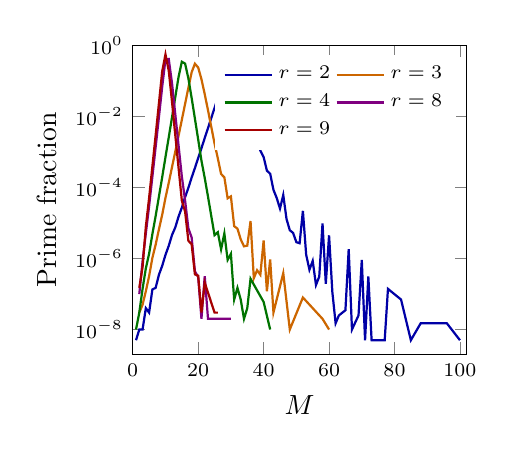
\begin{tikzpicture}
\begin{semilogyaxis}[width=0.48\textwidth,height=55mm,xlabel={$M$},ylabel={Prime fraction},xmin=0,xmax=102,ymin=2e-9,ymax=1,legend style={font=\scriptsize,draw=none},legend columns=2,legend pos=north east,tick label style={font=\scriptsize}]
\addplot+[no marks,line width=0.8pt,color=blue!65!black] coordinates {(1,4.9193177772e-09) (2,9.83863555441e-09) (3,9.83863555441e-09) (4,3.93545422176e-08) (5,2.95159066632e-08) (6,1.32821579985e-07) (7,1.47579533316e-07) (8,3.44352244404e-07) (9,6.14914722151e-07) (10,1.24950671541e-06) (11,2.25304754196e-06) (12,4.55036894391e-06) (13,7.43308916136e-06) (14,1.50481930805e-05) (15,2.68447171102e-05) (16,5.31089547227e-05) (17,9.70925749687e-05) (18,0.000190003729827) (19,0.000351613157443) (20,0.000673395571886) (21,0.00127596772573) (22,0.0024677659243) (23,0.00471604172801) (24,0.00905208583501) (25,0.0173928825933) (26,0.0336234337015) (27,0.0649021188584) (28,0.121780363087) (29,0.184933615282) (30,0.196312931971) (31,0.1513406174) (32,0.0958162579714) (33,0.0541449778045) (34,0.0290019166646) (35,0.0151560343648) (36,0.00804675437679) (37,0.00393201561864) (38,0.00204075438328) (39,0.00108657399131) (40,0.000718613940894) (41,0.000296369218805) (42,0.000243033975465) (43,8.56895963611e-05) (44,5.03688947208e-05) (45,2.53197285993e-05) (46,6.10782495218e-05) (47,1.28148228096e-05) (48,6.19834039928e-06) (49,5.21939616161e-06) (50,2.86304294633e-06) (51,2.66627023524e-06) (52,2.18270129775e-05) (53,1.26918398652e-06) (54,4.77173824389e-07) (55,8.46122657679e-07) (56,1.77095439979e-07) (57,3.04997702187e-07) (58,9.68613670332e-06) (59,1.91853393311e-07) (60,4.45690190615e-06) (61,1.13144308876e-07) (62,1.47579533316e-08) (63,2.4596588886e-08) (65,3.44352244404e-08) (66,1.80538962423e-06) (67,9.83863555441e-09) (69,2.4596588886e-08) (70,8.95315835451e-07) (71,4.9193177772e-09) (72,3.09917019964e-07) (73,4.9193177772e-09) (77,4.9193177772e-09) (78,1.37740897762e-07) (82,6.88704488809e-08) (85,4.9193177772e-09) (88,1.47579533316e-08) (96,1.47579533316e-08) (100,4.9193177772e-09)};\addlegendentry{$r=2$}
\addplot+[no marks,line width=0.8pt,color=orange!80!black] coordinates {(2,2.95164929849e-08) (3,4.91941549748e-08) (4,1.1806597194e-07) (5,3.14842591839e-07) (6,1.03307725447e-06) (7,2.44003008675e-06) (8,6.56250027364e-06) (9,1.69621446353e-05) (10,5.06011078071e-05) (11,0.000134437786715) (12,0.000373216376132) (13,0.00102011951405) (14,0.00285002401314) (15,0.00801473140616) (16,0.0226756226659) (17,0.064164851345) (18,0.176335986082) (19,0.306803371582) (20,0.240074294587) (21,0.111932887445) (22,0.0425776100025) (23,0.0149233125601) (24,0.00507636452951) (25,0.0017288990601) (26,0.000660175720931) (27,0.000238581812797) (28,0.00019232946829) (29,4.93220597778e-05) (30,5.58255270654e-05) (31,8.07768024687e-06) (32,6.88718169648e-06) (33,3.42391318625e-06) (34,2.18422048088e-06) (35,2.28260879083e-06) (36,1.12261061653e-05) (37,2.75487267859e-07) (38,4.62425056763e-07) (39,3.44359084824e-07) (40,3.17794241137e-06) (41,1.1806597194e-07) (42,9.34688944522e-07) (43,2.95164929849e-08) (46,3.83714408804e-07) (48,9.83883099497e-09) (52,7.87106479597e-08) (58,1.96776619899e-08) (60,9.83883099497e-09)};\addlegendentry{$r=3$}
\addplot+[no marks,line width=0.8pt,color=green!45!black] coordinates {(1,9.8388030191e-09) (2,2.95164090573e-08) (3,1.37743242267e-07) (4,5.21456560012e-07) (5,1.34791601362e-06) (6,4.83085228238e-06) (7,1.56535356034e-05) (8,5.48906820435e-05) (9,0.000194778783369) (10,0.000712004658083) (11,0.00256906888913) (12,0.00945309242434) (13,0.0348981654371) (14,0.129912273297) (15,0.349290671496) (16,0.309581469126) (17,0.118209656628) (18,0.0333621905426) (19,0.00865142675434) (20,0.00224669066941) (21,0.000566596988264) (22,0.000184202070124) (23,5.49792312707e-05) (24,1.56043415883e-05) (25,4.49633297973e-06) (26,5.45069687258e-06) (27,1.79066214948e-06) (28,5.0473059488e-06) (29,9.05169877757e-07) (30,1.3380772106e-06) (31,6.88716211337e-08) (32,1.47582045286e-07) (33,6.88716211337e-08) (34,1.96776060382e-08) (35,3.93552120764e-08) (36,2.65647681516e-07) (40,5.90328181146e-08) (42,9.8388030191e-09)};\addlegendentry{$r=4$}
\addplot+[no marks,line width=0.8pt,color=violet] coordinates {(2,9.83916081246e-08) (3,8.26489508247e-07) (4,5.01797201436e-06) (5,2.96552306888e-05) (6,0.000200502419036) (7,0.00137319263963) (8,0.00958623534462) (9,0.0684934091988) (10,0.402866112124) (11,0.417603089119) (12,0.0864349811921) (13,0.0116219380384) (14,0.00152569963222) (15,0.000204516796648) (16,4.27019579261e-05) (17,7.0251608201e-06) (18,3.87662936011e-06) (19,4.32923075748e-07) (20,2.95174824374e-07) (21,1.96783216249e-08) (22,3.14853145999e-07) (23,1.96783216249e-08) (24,1.96783216249e-08) (30,1.96783216249e-08)};\addlegendentry{$r=8$}
\addplot+[no marks,line width=0.8pt,color=red!65!black] coordinates {(2,1.47582585444e-07) (3,5.60813824687e-07) (4,7.82187702852e-06) (5,5.0532277256e-05) (6,0.000390828202772) (7,0.00296130360996) (8,0.0234051812586) (9,0.18654846128) (10,0.561564606815) (11,0.195670688469) (12,0.0260085970988) (13,0.00296570157101) (14,0.000355614997885) (15,4.25037846078e-05) (16,2.08386610647e-05) (17,3.12875081141e-06) (18,2.50890395254e-06) (19,3.54198205065e-07) (20,3.24681687976e-07) (21,2.95165170888e-08) (22,2.06615619621e-07) (25,2.95165170888e-08) (26,2.95165170888e-08)};\addlegendentry{$r=9$}
\end{semilogyaxis}\end{tikzpicture}\hfill
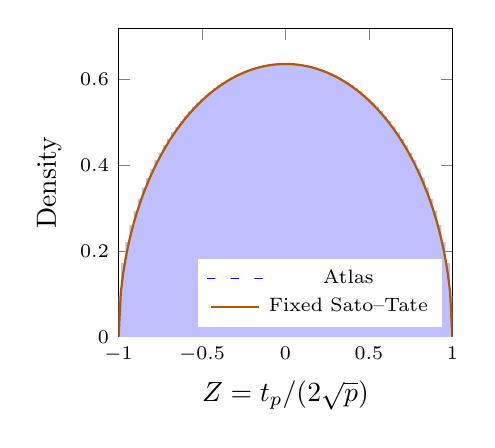
\begin{tikzpicture}
\begin{axis}[width=0.48\textwidth,height=55mm,xlabel={$Z=t_p/(2\sqrt p)$},ylabel={Density},xmin=-1,xmax=1,ymin=0,ymax=0.72,tick label style={font=\scriptsize},legend style={font=\scriptsize,draw=none},legend pos=south east]
\addplot+[ybar,bar width=2.7pt,no marks,draw=none,fill=blue!25] coordinates {(-0.9875,0.0944505082415) (-0.9625,0.171921695932) (-0.9375,0.220886617601) (-0.9125,0.260183505607) (-0.8875,0.29326867264) (-0.8625,0.322207838629) (-0.8375,0.347747362472) (-0.8125,0.371002551901) (-0.7875,0.391894894604) (-0.7625,0.411970630551) (-0.7375,0.429188833174) (-0.7125,0.447051859975) (-0.6875,0.46253472405) (-0.6625,0.477327702997) (-0.6375,0.490073458648) (-0.6125,0.503069115643) (-0.5875,0.515217075794) (-0.5625,0.526406949611) (-0.5375,0.536963018522) (-0.5125,0.546756789946) (-0.4875,0.556072993998) (-0.4625,0.564320131906) (-0.4375,0.572197730661) (-0.4125,0.580043649008) (-0.3875,0.586411410743) (-0.3625,0.593341745662) (-0.3375,0.599547760227) (-0.3125,0.604607967291) (-0.2875,0.609440508326) (-0.2625,0.614134127827) (-0.2375,0.618384024862) (-0.2125,0.621967846266) (-0.1875,0.625261034375) (-0.1625,0.628362172317) (-0.1375,0.630560517057) (-0.1125,0.632721081435) (-0.0875,0.634715569644) (-0.0625,0.63517818229) (-0.0375,0.636337370337) (-0.0125,0.636080778721) (0.0125,0.637039258601) (0.0375,0.635727965248) (0.0625,0.63551623781) (0.0875,0.634339733764) (0.1125,0.632112266664) (0.1375,0.630318093075) (0.1625,0.628323801639) (0.1875,0.625121916068) (0.2125,0.621989097719) (0.2375,0.618455453356) (0.2625,0.614745697416) (0.2875,0.609835037614) (0.3125,0.604881087815) (0.3375,0.599211672435) (0.3625,0.592929703603) (0.3875,0.587261075314) (0.4125,0.579999178376) (0.4375,0.572667623897) (0.4625,0.563780384357) (0.4875,0.555058827441) (0.5125,0.546587171868) (0.5375,0.536986040929) (0.5625,0.526353033888) (0.5875,0.515149385981) (0.6125,0.503128737775) (0.6375,0.49082454009) (0.6625,0.476728136543) (0.6875,0.461852316285) (0.7125,0.446847216354) (0.7375,0.429946408116) (0.7625,0.41200467223) (0.7875,0.39249465783) (0.8125,0.371197947204) (0.8375,0.347858735827) (0.8625,0.321577575632) (0.8875,0.293521328802) (0.9125,0.260378113819) (0.9375,0.220934236597) (0.9625,0.171937831295) (0.9875,0.0945673912325)};\addlegendentry{Atlas}
\addplot+[domain=-1:1,samples=151,no marks,thick,color=orange!70!black]{2/pi*sqrt(max(0,1-x^2))};\addlegendentry{Fixed Sato--Tate}
\end{axis}\end{tikzpicture}
\caption{Marginal maxima for selected orders and normalized elliptic traces in the full atlas. The trace comparator is fixed and has no fitted parameter.}\label{fig:atlas}
\end{figure}

The raw correlation between $A_4$ and $M_2$ is $0.531581$. Replacing
the quadruplet count by its normalized elliptic trace gives
$-0.002831$, or $-0.003086$ within the fifteen large-prime bands.
This removes the dominant prime-size trend; it does not prove
independence. There is a more basic obstruction to recovering a global
maximum from a short-pattern count. If $h_\ell$ counts maximal constant
runs of length $\ell$, then
\[
 A_k=\sum_{\ell\ge k}(\ell-k+1)h_\ell.
\]
A single weighted sum such as $A_4$ does not determine the farthest
nonzero entry of $h_\ell$.

\section{The fixed million ternary supplement}\label{sec:ternary}
\subsection{A separate population and three different counts}
The repository also contains a fixed sample of $1\,000\,000$
ternary profiles on $[2^{33},2^{34})$. It is a supplement,
not an extension of the complete census below $2^{32}$.
There are four strata of $250\,000$ primes each: the two
bands $[2^{33},3\cdot2^{32})$ and
$[3\cdot2^{32},2^{34})$, each divided according to whether
two is a cube. The equal sample weights differ from the
asymptotic natural relative cube-class density $1/3$.
No average with these four equal weights is presented as
a uniform prime average over the whole band.

For a prime $p$ in the supplement put $h=(p-1)/2$.
Reflection $x\mapsto p-x$ preserves the cubic character.
An ordinary canonical run is a maximal constant interval
strictly inside this half-period; it excludes the initial
run and the merged central run. Let $N_{p,k}$ count these
ordinary runs of length at least $k$, and let $C_p$ be
the full length of the central run. Then the predecessor
start count on the unfolded interval is
\begin{equation}\label{eq:ternary-starts}
 Z_{p,k}=2N_{p,k}+\mathbf1_{L_p\ge k}+\mathbf1_{C_p\ge k}.
\end{equation}
Here the predecessor ranges over $1,\ldots,p-k-1$.
The initial run at one has no predecessor, whereas its
reflected copy does; a central run has one start.
Overlapping $k$-windows inside a longer run are a third
observable and must not be substituted for $N_{p,k}$.

The stored thresholds are 18 through 27. The supplement
contains $33\,257\,058$ canonical maximal runs of length
at least 18, and $1\,235\,473$ retained canonical
positions at length at least 21. Exactly $1\,234\,808$
of the latter are ordinary. The difference is accounted
for by the prefix and centre conventions. Full-million
positions of lengths 18 through 20 were not retained.
The stored central field is zero below length 18; it does
not assert that the central run is absent.

At threshold 21, $299\,150$ profiles satisfy the interior
criterion $M<21$, while $293\,872$ satisfy both Rabung
criteria $K\le21$. For these primes
$K=\max(M+1,2L+2)$, consistent with
Section~\ref{sec:atlas}. Supplement membership includes
earlier diagnostic primes and is not an independent
validation of the analyses subsequently made on it.
The fixed selection and its scientific commitments
are documented in \path{data/ternary-million/}.

\subsection{Intensity, continuation, and a fixed comparator}
For an independent word of $h$ uniform $r$-colours,
the expected number of strictly interior maximal runs
of length at least $k$ is, for $k\le h-2$,
\begin{equation}\label{eq:iid-ordinary}
 \mu_{h,k}=\frac{(r-1)(h-k-1)-1}{r^k}+r^{1-h}.
\end{equation}
For proof, an interval of exact length $\ell$ has
probability $(r-1)^2/r^{\ell+1}$ of being constant
and different from its two neighbours. There are
$h-\ell-1$ interior placements; summing over
$k\le\ell\le h-2$ gives \eqref{eq:iid-ordinary}.
The formula retains the finite-word endpoints.
The tiny terminal term is omitted only when an
explicit bound or a cancelling equal-weight contrast
allows it.

Observed counts, their continuation from one threshold
to another, and the number of profiles with zero count
describe different features. For thresholds $a<b$,
the independent reference has geometric continuation
$3^{a-b}$, but the actual terminal and length corrections
must still be respected. A raised continuation rate can
decrease a void probability, while concentration of the
same total on fewer primes can increase it.
An unconditioned void deficit alone is therefore not a
proof of repulsion.

Conditioning a thinning model on its observed total
also changes its meaning. If $A$ initial objects are
allocated in groups and exactly $B$ survive, the
conditional count in a group of size $n$ is
hypergeometric:
\[
 \Prob(T=t\mid B)=
 \frac{\binom nt\binom{A-n}{B-t}}{\binom AB}.
\]
This describes an allocation model with the total
learned from the same sample. Even a close fit of that
conditional comparator does not estimate the
unconditional first intensity or prove a Poisson
law. We retain this distinction in reporting
the arithmetic contrasts below.

\subsection{A bounded arithmetic catalogue}
For each stored ordinary interval $[x,x+\ell-1]$,
the wide quadratic catalogue asks whether it contains
a position $y$ satisfying
\[
 (2y+A)^2\equiv D\pmod p,\qquad
 |A|\le128,\quad0<|D|\le4096,\quad
 D\notin\Q^2,\quad D\equiv A^2\pmod4.
\]
This is a root of the integer polynomial
$X^2+AX+(A^2-D)/4$ anywhere in the run,
not necessarily at its first position.
The rational catalogue asks whether the complete
interval contains a reduced cut $ap/q$ with
$2\le q\le128$.
The cut is nonintegral at these primes, so the
two neighbouring integer positions must both
belong to the interval. These parameter bounds
are fixed catalogue limits, not an assertion that
all possible arithmetic structures were found.

The CPU classification of all $1\,234\,808$
ordinary runs gives $1\,994$ wide quadratic hits
and 306 rational hits. Their union has 2300 runs
on 2187 primes. The two categories happen to be
disjoint in this extraction; the implementation
computes their union and does not rely on that
being a general property.
Among the quadratic hits, internal cubic
identities force two to be a cube for 1856 runs,
force the constant phase to be neutral for 1935,
and prove both conditions for 1855.
These are necessary-condition certificates,
not exact Kummer density calculations for
each detected model.

Removing only this fixed union moves the
prime-size-corrected cube/noncube contrast by
60.53\% at threshold 21, 52.86\% at 24,
and 83.93\% at 27. For the continuation
24 to 27, its contrast moves from 217 to
$563/27$, about 20.852, in units of the
cumulative half-million counts.
This is a finite descriptive decomposition
after model selection. It is not a causal
percentage explained or a prospective test.

\subsection{Applying the same filter to independent colours}
Removing an arithmetic catalogue from the observed
word requires evaluating that very same filter
in its comparator. Here the prime and its coordinate
mask are kept fixed and only its colours are
replaced by independent uniform colours.
The mask marks a complete maximal run if it meets
any allowed quadratic position or contains
any allowed rational cut; it is not truncated
to its first $k$ letters.

There is a useful exact finite geometry formula.
Remove the marked vertices and cut edges from
the interior positions $[2,h-1]$, and let
$L_1,\ldots,L_s$ be the remaining component lengths.
For $L\ge k$ define
\[
 F_{k,r}(L)=
 \frac{(r-1)(L-k+1)-1}{r^k}+r^{-L-1},
 \qquad F_{k,r}(L)=0\quad(L<k).
\]
If $T_{p,k}$ is the count marked by the filter,
then
\begin{equation}\label{eq:same-filter}
 \EE_{\rm iid}T_{p,k}
 =F_{k,r}(h-2)-\sum_{j=1}^sF_{k,r}(L_j).
\end{equation}
Indeed, for every exact length $\ell$ the number
of marked interior placements is
$(h-\ell-1)-\sum_j(L_j-\ell+1)_+$.
Multiplying by $(r-1)^2/r^{\ell+1}$ and summing
proves \eqref{eq:same-filter}. Components are
used to count placements; the observed word is
never shortened or concatenated.

For the wide mask there are 4032 nonsquare
discriminants. In one half-period, each
splitting discriminant gives at most one
interval of 128 or 129 marked vertices,
since its allowed $A$ values advance by two.
For $p>20996$ these intervals avoid the
word endpoints. Their total length is at
most 518112, and there are 2510 rational
cuts. Thus the number of intervals plus
cuts is at most 6542. In general, if total
marked length is at most $B$ and this
number is at most $J$, coverage of an
exact $\ell$-interval is bounded by
$B+(\ell-1)J$. Summing gives the uniform
bound
\[
 \EE_{\rm iid}T_{p,k}\le
 \frac{(r-1)(B+(k-1)J)+J}{r^k}.
\]
Using the same word lengths for all sampled
primes therefore gives:
\begin{center}
\begin{tabular}{r rr}
\toprule
$k$&Observed marked runs&Upper bound for iid expected total\\
\midrule
21&2300&124.703820\\
24&682&4.757640\\
27&228&0.181357\\
\bottomrule
\end{tabular}
\end{center}
The decimal upper bounds are rounded upwards.
They compare counts with bounded expectations;
they are not $p$-values.

The continuation correction admits a sharper signed
bound. Adding one letter to the length of a
test interval increases its covered placements
by a number between zero and $J$, apart from
the final finite-word cutoff. Summing these
increments gives, per profile,
\[
 -\frac{(r-1)(b-a)}{r^b}
 \le \EE_{\rm iid}T_{p,b}
       -r^{a-b}\EE_{\rm iid}T_{p,a}
 \le\frac{J(r-1)(b-a)}{r^b}.
\]
The same bounds applied to the two equal-sized
cube/noncube populations give an absolute
iid contrast below 0.002575 for 24 to 27.
After subtracting this background, the marked
catalogue accounts for a fraction between
90.389665\% and 90.392038\% of the initial
contrast 217; the centred residual lies in
$[20.849277,20.854427]$ cumulative occurrences.
These are outward-rounded rigorous enclosures
for the fixed comparator, not bounds for the
error of a universal maximum law.

\subsection{A separate fixed-length elliptic contribution}
The companion manuscript~\cite{cubiccompanion}
studies the cubic window count
$A^{(3)}_{p,4}$ on $1,\ldots,p-1$.
It proves an exact six-curve formula and
four vertical moments for
$(27A^{(3)}_{p,4}-p)/\sqrt p$.
Its conditional second moments are 44
when three is a cube and 17 otherwise;
the unconditional second and fourth
moments are 26 and 1900.
The conditioning concerns three, whereas
the present supplement is stratified by two.
The principal proof and its external analytic
inputs are in that companion.

The new oracle is useful as an exact
short-pattern cross-check. It neither
replaces the atlas's quadratic A4 column
nor reconstructs the maximum. In particular,
fixed-length trace moments do not close
the first intensity or the void probability
for logarithmically long cubic runs.

\section{Structural classification of extreme witnesses}\label{sec:classification}
\subsection{Boundary structure and rational anchors}
The neutral prefix is constrained by multiplicativity. In particular,
$L_r(p)+1$ must be prime: if it were composite, all its prime factors
would already be neutral, giving a contradiction. A related identity
describes half-word suffixes. Let $h=(p-1)/2$, and extend $\chi$ by
$\chi(0)=0$ when needed. Let $q$ be the least odd prime whose character
is not $1$. Then
\[
 \chi(h-j)=\sigma\chi(2)^{-1}\chi(2j+1).
\]
Every positive odd integer below $q$ is neutral, so the suffix of
$1,\ldots,h$ has length $(q-1)/2$. If $\sigma=1$, reflection joins
the two half-word suffixes into a central run of length $q-1$.
If $\chi(2)=1$, the ordinary neutral prefix ends at $q-1$; otherwise
it has length $1$. This explains long prefix and centre events without
a random-sign hypothesis.
The atlas has $L_8\ge2$ at approximately $24.9983\%$ of admissible
primes, instead of the naive $1/8$. For $p\equiv1\pmod8$, quadratic
reciprocity gives $(2/p)=1$, hence $\chi_{p,8}(2)^4=1$. The possible
values already lie in a subgroup of size four. This arithmetic
restriction illustrates why an independent-colour prefix model can
fail even before examining extreme runs.

A rational anchor $w$ can similarly place small rational multiples of
consecutive offsets close to fractions of $p$. The resulting signs are
controlled by a few small integers. An algebraic anchor instead
satisfies $P(w)=0\pmod p$ for a low-degree polynomial $P$; exact
identities in $\Q[X]/(P)$ then transfer to the residue window.
A polynomial congruence alone is not a compression explanation. It
must produce a smaller character-class group or another proved
constraint. The distinction is visible in a retained quartic at
$p=2\,654\,052\,683$, whose constant-window rank saves no condition.

Non-monic templates also enlarge the search class. For
$P=aX^2+bX+c$ and $\beta=a\alpha$,
\[
 \beta^2+b\beta+ac=0,\qquad
 \alpha+j=(\beta+aj)/a.
\]
The monic integral equation now has step $a$ rather than step one.
Scaling all positions preserves a constant colour but can change
whether that colour is neutral. A search restricted to integral
monic polynomials with unit-step windows need not include these
non-monic families~\cite{review4}.


\subsection{The selected deep tail}
The exploratory classification uses order-specific cutoffs
\[
 (52,36,28,26,26,22,20,20)\quad\text{for }r=2,\ldots,9.
\]
It selects $11\,557$ profiles and their canonical witnesses. The
first classification, before the higher-degree extensions, is printed
in Table~\ref{tab:classification}. Categories are assigned in order;
they are a reproducible bookkeeping scheme, not mutually exclusive
arithmetic possibilities in nature.
\begin{table}[htbp]\centering\small\setlength{\tabcolsep}{4pt}
\caption{Initial deep-tail classification, before the higher-degree extensions. The final unmodelled list is smaller, as described in the text.}\label{tab:classification}
\begin{tabular}{rrrrrrr}
\toprule
$r$ & Cutoff & Prefix/centre & Rational & Quadratic & Cubic & Remaining \\
\midrule
2 & 52 & 7675 & 430 & 531 & 6 & 44 \\
3 & 36 & 1538 & 26 & 170 & 1 & 0 \\
4 & 28 & 573 & 24 & 203 & 1 & 9 \\
5 & 26 & 118 & 1 & 58 & 0 & 0 \\
6 & 26 & 43 & 0 & 4 & 0 & 0 \\
7 & 22 & 36 & 1 & 9 & 0 & 0 \\
8 & 20 & 12 & 1 & 22 & 0 & 0 \\
9 & 20 & 7 & 1 & 13 & 0 & 0 \\
\bottomrule\end{tabular}\end{table}

The first stage left $53$ profiles: $44$ at order two and nine at
order four. Subsequent bounded searches retained models for fifteen
and then seven additional binary profiles, and for eight order-four
profiles. The remaining list has $23$ entries: $22$ binary profiles
and one order-four profile. This count includes the distinction just
made between a retained algebraic model and actual compression;
it should not be read as a theorem that all other profiles have one
unique explanation.

The $56$ deepest order-eight and order-nine profiles consist of $19$
prefix/centre cases, two rational cases, and $35$ quadratic cases.
The latter use square classes
$-47,-31,-23,33,73,97,145,148$ with respective multiplicities
$1,4,2,1,10,14,2,1$. After boundary and rational cases are removed,
the neutral shares rise sharply in the extreme tails: at order eight
they are $612/1767$ for $M\ge16$, $97/117$ for $M\ge18$, and $22/22$
for $M\ge20$; at order nine they are $202/340$, $52/53$, and $13/13$.
After the retained quadratic families are also removed at $M\ge16$,
the shares become $181/1327$ and $14/152$. These contrasts suggest a
mixture of ordinary bulk behaviour and special arithmetic families.
Because the families were found from these data, the contrasts are
descriptive evidence and not significance tests.

\section{Exact character-class certification}\label{sec:certification}
\subsection{Neutral and constant windows}
Let $F$ contain $\mu_r$, let $\alpha$ be a specified algebraic root,
and set $a_j=\alpha+j$ for $0\le j<m$, assuming $a_j\ne0$. Define
\[
 H_n=\langle[a_0],\ldots,[a_{m-1}]\rangle
       \subset F^\times/F^{\times r},\qquad
 H_c=\left\langle\left[\frac{a_j}{a_0}\right]:1\le j<m\right\rangle.
\]
The neutral event requires all characters to equal $1$; the constant
event only requires the ratios to be neutral. Kummer theory gives
the respective extension degrees $|H_n|$ and $|H_c|$. The quotient
$H_n/H_c$ is cyclic, generated by $[a_0]$, and its order is the number
of compatible constant phases. It can be $1$, $2$, or $4$ in an
order-four family. For several roots, the ratio construction is made
\emph{separately at every root}; different roots need not have the
same constant phase.

At order four, cardinalities must be computed over $\Z/4\Z$, not
inferred from a binary rank. An image generated by multiplication by
$2$ has order $2$, although its reduction modulo $2$ is zero.
We record groups as $C_4^a\times C_2^b$, with order $2^{2a+b}$.

\subsection{Matching upper and lower bounds}
Two certification paths are used. The earlier quadratic templates
use exact multiplicative decompositions in certified number fields,
with PARI's unconditional \texttt{bnfcertify(bn)} call. The higher
templates do not require a complete class group or a full basis of
$S$-units. They use the following elementary principle.
\begin{lemma}\label{lem:sandwich}
Let $H$ be generated by specified classes in $F^\times/F^{\times r}$.
Suppose explicit identities give a finite presentation mapping onto
$H$, of order at most $U$. Character homomorphisms at suitable finite
places give an image of order $L$. If $L=U$, then $|H|=L=U$ and the
presentation is exact.
\end{lemma}
\begin{proof}
The first map gives $|H|\le U$, and the second gives $L\le|H|$.
If a product of the radicandes, all units at the place, is an $r$th
power, its root has valuation zero and its reduction is an $r$th
power. Hence the finite-place characters respect every actual
relation and do descend to $H$.
\end{proof}
In the new order-four certificates, finite character matrices produce
a candidate kernel over $\Z/4\Z$. Every generator of that kernel is
then proved to be a fourth power in the specified field, with its
fourth root displayed in a rational power basis. This proves the
upper bound. Recomputing the character matrix proves the matching
lower bound. The auxiliary primes are homomorphism certificates,
not samples from which a rare-event frequency is estimated.

Irreducibility and Galois groups are separately established by
factorizations at unramified small primes. For cubics, cycle types
$3$ and $(1,2)$ force $S_3$. For the quartics considered here,
types $4$ and $(1,3)$ force $S_4$. The full roots, an explicit
square root of $-1$, and the appropriate degree prove the splitting
field composita used for the order-four calculations. A pair field
also carries an inverse of the difference of its two marked roots.
All identities are checked using rational quotient-field arithmetic
independent of PARI's power-search routines.

The finite computations can be large even when a density is tiny.
The largest new fields have degree $48$. Every PARI call had a
$30$-second deadline. A first batch containing several fourth-power
searches timed out and was not accepted. Balancing the exponents in
$\{-2,-1,0,1\}$ and certifying one generator per call gave complete
certificates. No approximation enters this change of representation.

\section{Prime densities through root orbits}\label{sec:orbits}
\subsection{A general inclusion--exclusion formula}
Put $C=\Q(\zeta_r)$. Let $N/C$ be a splitting field with Galois group
$\Gamma$, acting on roots $\alpha_1,\ldots,\alpha_d$. For a nonempty
root subset $S$, define
\[
 F_S=C(\alpha_i:i\in S),\qquad
 E_S=F_S(\sqrt[r]{\alpha_i+j}:i\in S,0\le j<m),
 \qquad h_S=[E_S:F_S].
\]
For constant windows replace each marked-root family by its own ratios.
All primes in this section are good primes, excluding the finite
ramification and non-unit exceptions.
\begin{proposition}\label{prop:orbit}
Among rational primes $p\equiv1\pmod r$, the limiting density that
at least one rational root has the required window is
\begin{equation}\label{eq:orbit}
 \delta=\sum_{S\ne\varnothing}
       \frac{(-1)^{|S|+1}}{[F_S:C]h_S}.
\end{equation}
When subsets are grouped into $\Gamma$-orbits, an orbit represented
by $S$ has positive coefficient
\[
 \frac{|\operatorname{Orb}(S)|}{[F_S:C]}
 =\frac{|\Stab_{\rm point}(S)|}{|\Stab_{\rm set}(S)|}.
\]
If the indicated action persists over $C$, the density among all
rational primes is $\delta/\varphi(r)$.
\end{proposition}
\begin{proof}
Take a common Galois extension containing all roots and radicals.
Fixing every root in $S$ and making its required characters neutral
is exactly the condition that Frobenius fix $E_S$ pointwise. This
subgroup has proportion $1/([F_S:C]h_S)$. Inclusion--exclusion of
the root events gives the stated group average, which is a central
function. Chebotarev gives its limiting prime average. The orbit
coefficient follows by orbit--stabilizer. Pointwise stabilization,
not setwise stabilization, supplies the root-field degree.
\end{proof}
Thus an existence probability is not the probability at one marked
root, and it is not generally the sum of the root probabilities.
Changing from neutral to constant windows requires different groups;
it cannot always be achieved by multiplying a neutral density by a
number of phases.

\subsection{Symmetric actions and root-count laws}
If $\Gamma=S_d$ and all size-$k$ subsets have a common group order
$h_k$, then
\begin{equation}\label{eq:Sn}
 \delta_{S_d}=\sum_{k=1}^d\frac{(-1)^{k+1}}{k!h_k}.
\end{equation}
Indeed $[F_S:C]=d!/(d-k)!$ and there are $\binom dk$ such subsets.
For $d=2,3,4$, respectively,
\[
 \delta_2=\frac1g-\frac1{2h_2},\qquad
 \delta_3=\frac1g-\frac1{2h_2}+\frac1{6h_3},
\]
\[
 \delta_4=\frac1g-\frac1{2h_2}+\frac1{6h_3}-\frac1{24h_4}.
\]
If $Z$ is the number of realizing rational roots, its binomial
moments are $s_k=\EE\binom Zk=1/(k!h_k)$, and
\begin{equation}\label{eq:rootlaw}
 \Prob(Z=j)=\sum_{k=j}^d(-1)^{k-j}\binom kj s_k,
 \qquad s_0=1.
\end{equation}
For all rational primes, divide the positive moments by
$\varphi(r)$ while retaining $s_0=1$. This also gives the mass at
zero for primes outside the admissible congruence class.

The field in which $h_k$ is calculated is part of the statement.
For $S_4$, a pair field has degree $12$ over $C$, while the normal
field has degree $24$. Extending a field can turn a nontrivial
radicand class into a power. Using its group order in the larger
field without checking this loss can give an incorrect density.
Our new quartic $h_2$ values are certified in the pair fields
themselves; $h_3$ and $h_4$ use the normal fields.

\section{Quadratic propagation and conjugate overlap}\label{sec:quadratic}
Consider
\[
 Q(X)=X^2+31X+216,
 \qquad A_j=\alpha+j\text{ in }\Q[\alpha]/(Q).
\]
It was motivated by an order-nine maximum at
$p=569\,704\,789$ with witness $w=77\,806\,457$.
\begin{theorem}\label{thm:propagation}
Let $p>512$, $Q(w)=0\pmod p$, and let $\chi$ be a character with
$\chi(-1)=1$. If $\chi(w+j)$ has one constant value for
$0\le j\le10$, that value and the characters of $2,3,11$ are $1$.
There is $t$ with $t^2=1$ such that the $26$ signs are
\[
 \chi(w+j)=
 \begin{cases}
 1,&0\le j\le10\text{ or }21\le j\le25,\\
 t,&11\le j\le20.
 \end{cases}
\]
For every odd character order, all $26$ values are therefore neutral.
\end{theorem}
\begin{proof}
Every identity in Table~\ref{tab:propagation} is an exact polynomial
identity after reduction modulo $Q$. Write $u_j=\chi(w+j)$,
$c=u_0=\cdots=u_{10}$, $a=\chi(2)$, and $b=\chi(3)$.
The first six identities give
\[
 u_{22}=1,\quad c=a^4,\quad u_{24}=a,
 \quad u_{21}=a^2/c,\quad u_{23}=a,\quad b=a.
\]
The additional identity $A_9A_{22}=-18$ gives $c=ab^2=a^3$.
Hence $a=b=c=1$. The eighth identity gives $\chi(11)=1$.
The first eight also determine $u_{21},\ldots,u_{25}=1$.
The ninth gives $u_{12}^2=1$, and identities ten to eighteen give
the same value $t=u_{12}$ at all positions $11,\ldots,20$.
For an odd order, $t^2=t^r=1$ implies $t=1$.
Finally $0<|Q(-j)|\le216$ at $0\le j\le31$. Such a modular root
cannot be within $31$ positions of zero at either ordinary boundary
when $p>512$, so all windows used here are ordinary and nonzero.
\end{proof}
\begin{table}[htbp]\centering\small\setlength{\tabcolsep}{4pt}
\caption{Exact propagation identities in $\Q[X]/(X^2+31X+216)$. Add $A_9A_{22}=-18$ to force the constant phase.}\label{tab:propagation}
\begin{tabular}{rl}
\toprule
Step & Identity \\
\midrule
1 & $A_{10}A_{22}=A_4$ \\
2 & $A_7A_8=-16A_{10}$ \\
3 & $A_9A_{24}=2A_0$ \\
4 & $A_8A_{21}=-2A_{24}$ \\
5 & $A_{10}A_{23}=2A_7$ \\
6 & $A_7A_{21}=-3A_{23}$ \\
7 & $A_9A_{25}=3A_3$ \\
8 & $A_3A_6=-22A_9$ \\
9 & $A_{12}^2A_{21}=-2A_0$ \\
10 & $A_{12}A_{18}=-A_0$ \\
11 & $A_{12}A_{20}=A_{24}$ \\
12 & $A_{10}A_{20}=-A_{16}$ \\
13 & $A_{11}A_{18}=-2A_9$ \\
14 & $A_{11}A_{19}=-A_7$ \\
15 & $A_{11}A_{21}=A_{15}$ \\
16 & $A_{10}A_{19}=-2A_{13}$ \\
17 & $A_{12}A_{17}=-2A_6$ \\
18 & $A_{14}A_{15}=-2A_3$ \\
\bottomrule\end{tabular}\end{table}

The parity qualification is necessary. At $p=98\,641$, with $r=2$
and $w=28\,104$, one obtains the pattern
$+^{11}-^{10}+^5$, although $\chi(-1)=1$.
At order nine, the ten positions
$\{0,1,2,3,4,5,6,7,9,10\}$ suffice to enforce neutrality of all
$26$. The independent exact group is $C_9^{10}$, so ten is also
minimal among tests supplied by a generating set of individual
radicand classes. This does not bound arbitrary algorithms using
other information. The earlier determinant certificate has absolute
determinant $10$ for these ten positions and is invertible modulo $9$;
the constant-phase system has absolute determinant $2$ and explains
the order-two obstruction in Theorem~\ref{thm:propagation}.

Three further identities are
\[
 A_{27}A_4=-108,\qquad A_{28}A_3=-132,\qquad A_{31}A_0=-216.
\]
They make positions $27,28,31$ neutral in the odd-order case. If
position $26$ is neutral, the local run has at least $29$ positions;
stops at lengths $27$ or $28$ are impossible for this template.
None of these assertions identifies a prime's global maximum.

The conjugate root is $w'=-31-w$. For odd orders,
$\chi(w'+j)=\chi(w+31-j)$. Thus the two neutral windows of length
$26$ cover positions $0,\ldots,31$ at either root. Conversely, a
neutral $32$-window yields both $26$-windows. With $r=9$, the exact
group orders are $g_{26}=9^{10}$ and $h_{26}=9^{13}$. Consequently,
among admissible primes,
\[
 \delta_{26}=\frac{1457}{2\cdot9^{13}},\qquad
 \delta_{29}=\frac{161}{2\cdot9^{13}},\qquad
 \delta_{32}=\frac1{2\cdot9^{13}}.
\]
Therefore $\Prob(A_{32}\mid A_{26})=1/1457$ and
$\Prob(A_{32}\mid A_{29})=1/161$. These count primes with at least
one realization. The continuation probability from $26$ to $29$
at a \emph{marked root} is instead $1/9$; it answers a different
question. Appendix~\ref{app:quadratics} gives all seventeen certified
quadratic density parameters.

\section{A length-53 cubic as a binary code}\label{sec:code}
\subsection{Complete relations and the arithmetic population}
Let
\[
 f(X)=X^3+163X^2+8010X+121176,
 \qquad \alpha\in\Q[X]/(f),\quad A_j=\alpha+j.
\]
This family arose at $p=3\,836\,617\,441$ in the quadratic atlas.
The group generated by its $53$ radicandes has dimension $41$ over
$\Ftwo$. Its ratio group has dimension $40$, so both constant signs
are possible. Twelve independent square identities give an upper
bound; finite-place character rows of rank $41$ give the matching
lower bound. The relations can be chosen with four supports of
weight $4$ and eight of weight $6$, total weight $64$. All $4096$
linear combinations have the weight distribution in
Table~\ref{tab:dual}. The four weight-$4$ relations are independent,
and weights at most $6$ span the complete relation space. Hence
$64$ is the least possible total weight of a relation basis, a
statement about this criterion rather than universal computational
optimality.
\begin{table}[htbp]\centering\small\setlength{\tabcolsep}{4pt}
\caption{Weight distribution of all $4096$ relations in the length-$53$ cubic.}\label{tab:dual}
\begin{tabular}{rrrrrrrrrrrr}
\toprule
Weight & 0 & 4 & 6 & 8 & 10 & 12 & 14 & 16 & 18 & 20 & 22 \\
\midrule
Count & 1 & 4 & 33 & 183 & 514 & 1003 & 1118 & 832 & 346 & 57 & 5 \\
\bottomrule\end{tabular}\end{table}

Let $R$ be a matrix of these twelve supports. Encode a sign as
$(-1)^{x_j}$ and define
\[
 \mathcal C=\{x\in\Ftwo^{53}:Rx=0\}.
\]
This is a binary code of dimension $41$.
\begin{proposition}\label{prop:uniformcode}
In the population of all pairs $(p,w)$ with $p\le X$ a good prime
and $f(w)=0$ in $\Fp$, the relative frequency of each sign vector
in $\mathcal C$ tends to $2^{-41}$ as $X\to\infty$.
\end{proposition}
\begin{proof}
Take a Galois extension containing the roots and the square roots
of every conjugate family. The stabilizer of one root projects
onto the Kummer group of its $41$ independent classes. Every
compatible sign vector has the same number of lifts in that
stabilizer. For a specified vector, sum the number of marked
rational roots carrying it over the conjugate roots. This is a
central function of Frobenius, and Chebotarev gives its group
average. Transitivity makes the mean number of rational roots
equal to one; equivalently, sum the sizes of the point stabilizers.
Normalizing by all prime/root pairs yields the stated uniform law.
\end{proof}
A prime with three rational roots contributes three pairs. This
population is neither a canonical-root sample nor a record-selected
sample. Additional congruence conditioning can also change the law.
No error term for $X=2^{32}$ is asserted.

\subsection{Three-wise independence and exceptional tails}
The dual code has no nonzero vector of weight $1$, $2$, or $3$.
Every projection of $\mathcal C$ onto at most three coordinates is
therefore uniform. These signs are independent up to triples in
the limiting population of Proposition~\ref{prop:uniformcode}.
They are not independent at all orders. The positions
$22,30,33,37$, for example, have a product identically equal to $+1$.
Both constant vectors belong to $\mathcal C$, so
\[
 \Prob(\text{all 53 signs constant})=
 \frac2{2^{41}}=2^{-40}.
\]
For $53$ independent fair signs this probability is $2^{-52}$.
Thus three-wise independence is compatible with an enhancement
factor $2^{12}=4096$ at this extreme.

The full weight law follows from MacWilliams' identity. If $B_w$
is the number of dual words of weight $w$, the number of code
words of weight $k$ is
\begin{equation}\label{eq:macwilliams}
 A_k=2^{-12}\sum_w B_w
       \sum_j(-1)^j\binom wj\binom{53-w}{k-j}.
\end{equation}
It was independently checked by literal enumeration of the
$2^{15}$ compatible words on the $27$ active coordinates and
convolution with the $26$ free coordinates. If $V$ counts negative
signs, its first four central moments are
\[
 0,\qquad \frac{53}{4},\qquad0,\qquad\frac{8417}{16}.
\]
The independent-sign fourth moment is $8321/16$, differing by $6$.

\subsection{The exact local longest-run law}
Weight counts alone do not determine run arrangement. The longest
constant segment inside this fixed $53$-window was computed by two
independent integer methods. A syndrome automaton retains the last
sign, current run length, and a $12$-bit relation syndrome. A Fourier
method uses
\[
 \mathbf1_{Rx=0}=2^{-12}\sum_{u\in\mathcal C^\perp}(-1)^{u\cdot x}
\]
and a signed last-sign/run-length recurrence for each dual word.
Both produce the same counts for all $54$ strict maximum thresholds.
They were also checked against literal enumeration on $21$ small
test codes. Figure~\ref{fig:code} and Table~\ref{tab:localtail} show
the difference from independent signs.
\begin{table}[htbp]\centering\small\setlength{\tabcolsep}{4pt}
\caption{Exact local longest-run tails in the fixed cubic window. Decimal columns approximate the exact counts.}\label{tab:localtail}
\begin{tabular}{rrrrr}
\toprule
$k$ & Certified probability & Decimal & Independent signs & Ratio \\
\midrule
10 & $95\,288\,989\,062/2^{41}$ & $0.0433324$ & $0.0433481$ & 0.9996 \\
26 & $2\,064\,382/2^{41}$ & $9.38772e-07$ & $4.32134e-07$ & 2.172 \\
40 & $896/2^{41}$ & $4.07454e-10$ & $1.36424e-11$ & 29.87 \\
52 & $2/2^{41}$ & $9.09495e-13$ & $6.66134e-16$ & 1365 \\
53 & $2/2^{41}$ & $9.09495e-13$ & $2.22045e-16$ & 4096 \\
\bottomrule\end{tabular}\end{table}

\begin{figure}[htbp]\centering
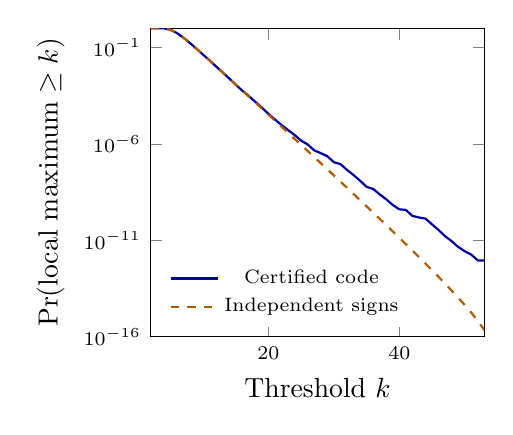
\begin{tikzpicture}
\begin{semilogyaxis}[width=0.48\textwidth,height=55mm,xlabel={Threshold $k$},ylabel={$\Prob(\text{local maximum}\ge k)$},xmin=2,xmax=53,ymin=1e-16,ymax=1,legend style={font=\scriptsize,draw=none},legend pos=south west,tick label style={font=\scriptsize}]
\addplot+[no marks,thick,blue!65!black] coordinates {(2,1) (3,0.999981142068) (4,0.985424262727) (5,0.839830755766) (6,0.567800115372) (7,0.325825781585) (8,0.172038583806) (9,0.0871545450045) (10,0.0433324153446) (11,0.021348276653) (12,0.0104648199622) (13,0.00511879158876) (14,0.00250037830847) (15,0.00118966036098) (16,0.000579683350225) (17,0.000305116875097) (18,0.000152573746163) (19,7.62871495681e-05) (20,3.62367391062e-05) (21,1.85958961083e-05) (22,9.53653398028e-06) (23,5.24518327438e-06) (24,2.920625775e-06) (25,1.49011520989e-06) (26,9.38772245718e-07) (27,4.61935997009e-07) (28,3.31550836563e-07) (29,2.30967998505e-07) (30,1.12690031528e-07) (31,9.03382897377e-08) (32,4.54019755125e-08) (33,2.44472175837e-08) (34,1.23982317746e-08) (35,5.93718141317e-09) (36,4.65661287308e-09) (37,2.44472175837e-09) (38,1.35332811624e-09) (39,6.83940015733e-10) (40,4.07453626394e-10) (41,3.78349795938e-10) (42,1.85536919162e-10) (43,1.52795109898e-10) (44,1.34605215862e-10) (45,6.73026079312e-11) (46,3.45607986674e-11) (47,1.63709046319e-11) (48,9.09494701773e-12) (49,4.54747350886e-12) (50,2.72848410532e-12) (51,1.81898940355e-12) (52,9.09494701773e-13) (53,9.09494701773e-13)};\addlegendentry{Certified code}
\addplot+[no marks,dashed,thick,orange!70!black] coordinates {(2,1) (3,0.999980844751) (4,0.985407012784) (5,0.839689395121) (6,0.567004855738) (7,0.325798675453) (8,0.172027101916) (9,0.0871957696287) (10,0.0433481495166) (11,0.021351093606) (12,0.0104685616528) (13,0.00512048747623) (14,0.00250103707231) (15,0.00122040138245) (16,0.000595028745284) (17,0.000289903604433) (18,0.000141141048516) (19,6.86639978085e-05) (20,3.33784928443e-05) (21,1.62124429153e-05) (22,7.86780941553e-06) (23,3.81469664035e-06) (24,1.84774389211e-06) (25,8.94069659196e-07) (26,4.32133673511e-07) (27,2.08616256714e-07) (28,1.00582838058e-07) (29,4.842877388e-08) (30,2.32830643654e-08) (31,1.11758708954e-08) (32,5.35510480404e-09) (33,2.56113708019e-09) (34,1.22236087918e-09) (35,5.82076609135e-10) (36,2.76486389339e-10) (37,1.30967237055e-10) (38,6.18456397206e-11) (39,2.91038304567e-11) (40,1.36424205266e-11) (41,6.36646291241e-12) (42,2.95585778076e-12) (43,1.36424205266e-12) (44,6.25277607469e-13) (45,2.84217094304e-13) (46,1.27897692437e-13) (47,5.68434188608e-14) (48,2.48689957516e-14) (49,1.06581410364e-14) (50,4.4408920985e-15) (51,1.7763568394e-15) (52,6.66133814775e-16) (53,2.22044604925e-16)};\addlegendentry{Independent signs}
\end{semilogyaxis}\end{tikzpicture}\hfill
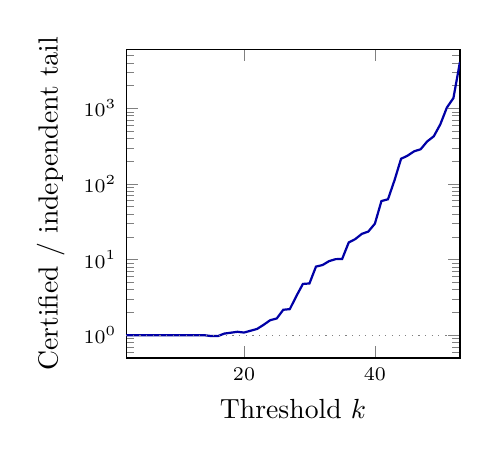
\begin{tikzpicture}
\begin{semilogyaxis}[width=0.48\textwidth,height=55mm,xlabel={Threshold $k$},ylabel={Certified / independent tail},xmin=2,xmax=53,ymin=0.5,ymax=6000,tick label style={font=\scriptsize}]
\addplot+[no marks,thick,blue!65!black] coordinates {(2,1) (3,1.00000029732) (4,1.0000175054) (5,1.00016834873) (6,1.0014025623) (7,1.00008319902) (8,1.00006674466) (9,0.999527217612) (10,0.999637027827) (11,0.999868065166) (12,0.999642578351) (13,0.999668803511) (14,0.999736603729) (15,0.974810728734) (16,0.974210665987) (17,1.05247699729) (18,1.08100193223) (19,1.11102108824) (20,1.08563137573) (21,1.14701382176) (22,1.21209519405) (23,1.37499354966) (24,1.58064425891) (25,1.66666567259) (26,2.17241169402) (27,2.21428571429) (28,3.2962962963) (29,4.76923076923) (30,4.84) (31,8.08333333333) (32,8.47826086957) (33,9.54545454545) (34,10.1428571429) (35,10.2) (36,16.8421052632) (37,18.6666666667) (38,21.8823529412) (39,23.5) (40,29.8666666667) (41,59.4285714286) (42,62.7692307692) (43,112) (44,215.272727273) (45,236.8) (46,270.222222222) (47,288) (48,365.714285714) (49,426.666666667) (50,614.4) (51,1024) (52,1365.33333333) (53,4096)};
\addplot+[domain=2:53,no marks,dotted,gray]{1};
\end{semilogyaxis}\end{tikzpicture}
\caption{Exact limiting local tails in the length-$53$ cubic code. The law concerns prime/root pairs for this fixed window, not canonical global maxima.}\label{fig:code}
\end{figure}
At threshold $10$ the two probabilities differ very little; at
$26$ the enhancement is about $2.17$, and at $40$ about $29.87$.
The tail becomes especially rigid at the end. The relations on
$\{36,37,46,52\}$ and $\{0,2,17,30,33,45\}$ force the missing endpoint
whenever $52$ consecutive signs are constant. Hence a local maximum
of exactly $52$ is impossible: every constant $52$-segment completes
to all $53$. This is a theorem about a fixed algebraic window, not
a gap theorem for the global maxima of arbitrary primes.

At the level of prime existence the same family has
\[
 \delta_n=2^{-41}-2^{-79}+\frac1{6\cdot2^{109}},\qquad
 \delta_c=2^{-40}-2^{-78}+\frac1{6\cdot2^{109}}.
\]
Thus $2\delta_n-\delta_c=1/(6\cdot2^{109})$. The constant density
is very close to twice the neutral density, but it is not equal
to it. Conjugate-root overlap supplies the correction.

\section{Higher-root dependencies explained by norms}\label{sec:norms}
\subsection{The two families and their dimensions}
The two newest binary families are
\begin{align*}
 P_3(X)&=X^3-197X^2-9264X-90252,&m&=53,\\
 P_4(X)&=X^4+100X^3+3258X^2+34844X+26309,&m&=52.
\end{align*}
Their originating primes are $1\,779\,238\,511$ and
$3\,173\,249\,399$; both observed phases are neutral. Their Galois
groups are $S_3$ and $S_4$. Work in their normal fields, and write
$H_i$ for the square classes generated by $\alpha_i+j$.
For $P_3$ the common rational subgroup is
\[
 C_3=\langle[2],[3],[5],[11],[17],[19],[59],[763]\rangle,
 \qquad\dim C_3=8.
\]
Each $H_i$ has dimension $51$, any pair has dimension $94$, and
the total has dimension $121$. After quotienting by $C_3$, each
block has dimension $43$, any two have dimension $86$, and the
sum has dimension $113$ rather than $129$.

For $P_4$, the common subgroup is
\[
 C_4=\langle[2],[3],[14]\rangle,\qquad\dim C_4=3.
\]
The one-, two-, three-, and four-root dimensions are respectively
$44,85,126,159$. A block modulo $C_4$ has dimension $41$; any
three sum directly to dimension $123$, but all four have dimension
$156$ rather than $164$.

\subsection{A norm description of every remaining relation}
For either monic polynomial, define the rational shifted norm
\[
 \nu_j=\prod_{i=1}^d(\alpha_i+j)=(-1)^dP(-j).
\]
Let $K$ be the space of binary relations among all $dm$ factors.
Let $K_0$ be generated by relations internal to one block and by
identifying the common rational classes between blocks.
\begin{theorem}\label{thm:norms}
For $P_3$, $K/K_0$ has dimension $16$; for $P_4$ it has dimension
$8$. In both cases this quotient is generated entirely by diagonal
norm constraints: products of shifted norms belonging to the
common rational subgroup. The Galois action on $K/K_0$ is trivial.
\end{theorem}
\begin{proof}
The earlier exact square identities and matching character ranks
certify the total relation spaces. Explicit square roots certify
the displayed rational classes as elements of each $H_i$.
The new verifier checks the dimensions of every proper subset
of the quotient blocks. The shifted norms span dimension $27$
modulo $C_3$ in the cubic case and dimension $33$ modulo $C_4$
in the quartic case. Thus their kernels modulo the single-block
relation spaces have dimensions $43-27=16$ and $41-33=8$.
Each kernel vector supplies the same factor support in every
block, followed by a common-class correction in the first block.
Its actual square relation is checked as a combination of the
archived exact square relations. These vectors are independent
modulo $K_0$ and reach the full respective deficits. They therefore
generate $K/K_0$. A root permutation preserves a diagonal norm
support; moving the common correction to another block changes
it only by a generator of $K_0$. Hence the quotient action is trivial.
\end{proof}
This is a description by exact generators and dimensions, not just
an observed correlation of residue signs. A short generating basis
is particularly transparent. For the cubic there are seven
single-position norm constraints, eight pairs, and one triple:
\[
\begin{split}
 &\{7\},\{10\},\{12\},\{13\},\{26\},\{27\},\{28\},\\
 &\{3,8\},\{3,9\},\{17,18\},\{17,19\},\{17,20\},
   \{15,22\},\{15,24\},\{33,48\},\{0,17,23\}.
\end{split}
\]
For the quartic the basis is
\[
 \{22\},\{29\},\{31\},\{37\},\{38\},\{41\},\{47\},\{25,39\}.
\]
For example, the cubic has
$\nu_7=35400$ and $354\nu_7=3540^2$, with
$354=2\cdot3\cdot59$ in its common subgroup. The quartic has
\[
 \nu_{47}=82944=288^2,
 \qquad\prod_{i=1}^4(\alpha_i+47)=288^2.
\]
This is a pure four-block relation. All basis relations are recorded
as integer-square identities, and none of these selected bases
needs a discriminant-class correction.

\subsection{Probabilistic consequences under an explicit conditioning}
Condition on the normal field splitting and on every common class
being neutral, and choose a place over the prime uniformly to label
the roots. The remaining Kummer character is uniform on the dual
of the quotient class group. In the cubic case any pair of
block sign vectors is independent, but all three are not. Their
individual neutral probabilities are $2^{-43}$, while simultaneous
neutrality is $2^{-113}$ instead of $2^{-129}$: a factor $2^{16}$.
In the quartic case any three block vectors are independent, while
all four neutral probabilities combine to $2^{-156}$ instead of
$2^{-164}$: a factor $2^8=256$.

These conclusions concern the stated splitting and common-neutral
population. They do not assert unconditioned pairwise independence
among the original atlas maxima. The full prime-existence densities
among all primes are
\[
 \delta(P_3)=2^{-51}-2^{-95}+\frac1{3\cdot2^{122}},
\]
\[
 \delta(P_4)=2^{-44}-2^{-86}
       +\frac1{3\cdot2^{127}}-\frac1{3\cdot2^{162}}.
\]
Neutral and constant modes coincide in these two families.
For the cubic this can also be seen from
\[
 A_3A_{12}A_{43}=255A_{15}A_{24},\quad
 A_{18}A_{27}A_{43}=285A_{15}A_{26},\quad
 A_{37}A_{43}A_{46}=323A_{22}A_{23}.
\]
Each identity constrains a constant phase to the character of its
coefficient. Since $255\cdot285\cdot323=4845^2$, the common phase
must be neutral. This compresses the phase argument without
discarding the full square-rank certificate.


\subsection{A parity normal form and the remaining information}
The received review~\cite{review4} suggests a useful linear description
of these dependencies. It is compatible with, but logically weaker
than, their explicit generation by norms.

\begin{lemma}\label{lem:parityform}
Let $V_1,\ldots,V_n$ be binary subspaces of dimension $d$, such that
every sum of $n-1$ of them is direct and
$\dim(V_1+\cdots+V_n)=nd-e$. There are bases in the individual
spaces for which compatible dual character coordinates satisfy
exactly
\[
 z_{1,j}+\cdots+z_{n,j}=0,\qquad 1\le j\le e.
\]
The other $n(d-e)$ coordinates are free. Under the uniform law on
the compatible characters, knowledge of $n-1$ blocks leaves
exactly $d-e$ free bits in the last block.
\end{lemma}
\begin{proof}
The kernel $R$ of the sum map $\bigoplus_iV_i\to\sum_iV_i$ has
dimension $e$. Its projection into every $V_i$ is injective:
a kernel vector with a zero $i$th component would be a relation
among the other $n-1$ spaces. Choose a basis $r_1,\ldots,r_e$ of
$R$. Its projected components are independent in each block;
complete them to a basis there. Annihilating the $r_j$ gives the
displayed $e$ parities, with no further relation. Each fixes one
coordinate of the final block once the other blocks are known.
\end{proof}

Apply the lemma to $V_i=H_i/C$ in the population specified above.
The cubic has $16$ three-block parities and $27$ bits left after
two block motifs are given. The quartic has $8$ four-block
parities and $33$ bits left after three motifs are given.
These are full admissible block motifs, not $43$ or $41$
independent original positions within a window.
Explicit basis changes derived from the certified character
groups are recorded in \texttt{VERIFICATION\_REPORT4.json}.
The linear normal form alone does not determine a Galois action;
the trivial action in these two examples is established separately
by Theorem~\ref{thm:norms} and its norm generators.

If $Z$ counts neutral blocks in this conditioned population, its
whole limiting law follows by the inversion in \eqref{eq:rootlaw}
from
\[
 \EE\binom Zk=\binom nk2^{-kd}\quad(1\le k<n),
 \qquad \EE\binom Zn=2^{-nd+e}.
\]
The supplied exact fractions distinguish this law from the
unconditioned prime-existence densities above.

\section{All eight new order-four density laws}\label{sec:order4}
The preceding residual study retained three quadratic, three cubic,
and two $S_4$ quartic models at order four. Their exact single-root
groups were already certified. The new calculation completes their
pair and higher-root groups and therefore their prime densities.
All relevant splitting actions are disjoint from $\Q(i)$, so the
action remains $C_2$, $S_3$, or $S_4$ over the cyclotomic base.
The largest normal composita have degree $48$ over $\Q$; the
quartic pair composita have degree $24$.

Table~\ref{tab:r4groups} gives every group cardinality needed for
\eqref{eq:Sn}. The numbers are base-two logarithms, so a row
$48,93,138,174$ means $g=2^{48}$, $h_2=2^{93}$,
$h_3=2^{138}$, and $h_4=2^{174}$. Every row is certified by
explicit fourth powers and matching characters. The neutral and
constant rows are separate, and the positive moments in
\eqref{eq:rootlaw} must be divided by two to count all primes.
\begin{table}[!htbp]\centering\small\setlength{\tabcolsep}{4pt}
\caption{The eight newly completed order-four templates. Coefficient vectors are in descending order.}\label{tab:r4poly}
\begin{tabular}{rrl}
\toprule
Originating prime & $m$ & Polynomial coefficients \\
\midrule
$1\,065\,972\,469$ & 28 & $(4,168,2485,15006,30001)$ \\
$1\,583\,868\,241$ & 28 & $(2,58,411)$ \\
$2\,400\,748\,661$ & 28 & $(5,117,640)$ \\
$2\,453\,400\,749$ & 28 & $(5,256,3707,16560)$ \\
$2\,789\,197\,129$ & 29 & $(5,255,2818,1848)$ \\
$3\,318\,080\,401$ & 29 & $(2,49,288)$ \\
$3\,832\,210\,429$ & 28 & $(9,493,8612,47628)$ \\
$4\,129\,372\,337$ & 28 & $(1,41,424,164,-8320)$ \\
\bottomrule\end{tabular}\end{table}
\begin{table}[!htbp]\centering\small\setlength{\tabcolsep}{4pt}
\caption{Exact base-two logarithms of subset group orders for every new order-four model. The pair fields are used for $h_2$.}\label{tab:r4groups}
\begin{tabular}{rrlrrrr}
\toprule
Originating prime & $m$ & Mode & $\log_2g$ & $\log_2h_2$ & $\log_2h_3$ & $\log_2h_4$ \\
\midrule
$1\,065\,972\,469$ & 28 & neutral & 48 & 93 & 138 & 174 \\
$1\,065\,972\,469$ & 28 & constant & 47 & 91 & 135 & 171 \\
$1\,583\,868\,241$ & 28 & neutral & 38 & 42 & -- & -- \\
$1\,583\,868\,241$ & 28 & constant & 36 & 40 & -- & -- \\
$2\,400\,748\,661$ & 28 & neutral & 34 & 52 & -- & -- \\
$2\,400\,748\,661$ & 28 & constant & 32 & 52 & -- & -- \\
$2\,453\,400\,749$ & 28 & neutral & 48 & 90 & 118 & -- \\
$2\,453\,400\,749$ & 28 & constant & 46 & 88 & 118 & -- \\
$2\,789\,197\,129$ & 29 & neutral & 53 & 101 & 134 & -- \\
$2\,789\,197\,129$ & 29 & constant & 51 & 98 & 132 & -- \\
$3\,318\,080\,401$ & 29 & neutral & 38 & 54 & -- & -- \\
$3\,318\,080\,401$ & 29 & constant & 37 & 54 & -- & -- \\
$3\,832\,210\,429$ & 28 & neutral & 54 & 104 & 140 & -- \\
$3\,832\,210\,429$ & 28 & constant & 52 & 102 & 140 & -- \\
$4\,129\,372\,337$ & 28 & neutral & 53 & 102 & 151 & 183 \\
$4\,129\,372\,337$ & 28 & constant & 51 & 100 & 149 & 183 \\
\bottomrule\end{tabular}\end{table}

For example, the neutral density of the first quartic is exactly
\[
 \frac12\left(2^{-48}-2^{-94}
                  +\frac1{6\cdot2^{138}}-\frac1{24\cdot2^{174}}\right).
\]
The table is an exact specification of all sixteen densities, rather
than decimal approximations to tiny numbers. The delivered JSON
also gives all binomial moments and the full laws for the number
of realizing roots, in both populations and both modes.

\subsection{Short phase identities and a 30-term continuation}
The quadratic phase coupling admits short identities, supplied
in the received review~\cite{review4} and independently checked
in the exact fields. Put $A_j=\alpha+j$ and
$B_j=\bar\alpha+j$ for the two roots of each quadratic.
For $2X^2+58X+411$ the identities are
\[
 A_9A_{11}=-A_{12}A_{26},\qquad
 A_{12}B_3=A_9A_{11}.
\]
The first shows that even \emph{one} constant 28-window forces
$\chi_{p,4}(-1)=1$, hence $p\equiv1\pmod8$.
The second forces two constant windows to have the same phase.
All four diagonal phase pairs $(1,1),(i,i),(-1,-1),(-i,-i)$
are permitted by the exact joint group. The congruence restriction
is already included in the density, so no additional factor of
$1/2$ is applied.

Here $\bar\alpha=-29-\alpha$. The two constant 28-windows
reflect to the intervals $0,\ldots,27$ and $2,\ldots,29$ at
$\alpha$. They therefore join to a constant 30-window.
Conversely, a constant 30-window supplies both 28-windows.
The statement holds for neutral windows as well.
For $p>1126$ the coefficient and quadratic discriminant
exceptions are absent, and $0<|P(-j)|\le411$ for $0\le j<30$
excludes a zero or an ordinary-boundary crossing.
The joined neutral group is $C_4^{21}$ and the joined ratio
group is $C_4^{20}$, exactly the two-root groups. The first
identity puts the class of $-1$ in the original neutral group,
so the reflected generators supply the last two positions.
For the ratio groups,
$B_j/B_0=A_{29-j}/A_{29}$ and
$A_{29}/A_0=(A_{26}/A_0)/(B_3/B_0)$, which identifies the
ratio groups. Among all rational primes the densities of this
particular 30-window event are
\[
 \delta_{30,n}=2^{-44},\qquad
 \delta_{30,c}=2^{-42},\qquad
 \Prob(A_{30,c}\mid A_{28,c})=\frac1{31}.
\]
Among admissible primes the first two values double.
A single 28-window need not continue: the extension is
equivalent to the two-root event, not forced by one root alone.

For $5X^2+117X+640$ and $2X^2+49X+288$, respectively, the
identities are
\[
 A_0B_{16}=16A_8,\qquad A_{10}B_{11}=A_9.
\]
Since $16=2^4$, two constant phases $\phi,\psi$ satisfy
$\phi\psi=\phi$, and hence $\psi=1$; conjugation gives
$\phi=1$. These identities explain why the two joint ratio
groups equal their neutral counterparts even though an isolated
constant window may be non-neutral.
The exact densities among all primes remain
\begin{center}
\begin{tabular}{lcc}
\toprule
Polynomial & Neutral density & Constant density\\
\midrule
$2X^2+58X+411$ & $31/2^{44}$ & $31/2^{42}$\\
$5X^2+117X+640$ & $524287/2^{54}$ & $2097151/2^{54}$\\
$2X^2+49X+288$ & $131071/2^{56}$ & $262143/2^{56}$\\
\bottomrule
\end{tabular}
\end{center}
The conditional probabilities of two realizing roots given at
least one constant realization are respectively
$1/31$, $1/2097151$, and $1/262143$.
In these three quadratic families a non-neutral constant root
cannot coexist with a neutral constant root. Thus subtracting
neutral from constant existence densities does count existence
of a non-neutral realization, with all-prime values
\[
 \delta_{\mathrm{nonneutral}}=
 \frac{93}{2^{44}},\qquad\frac3{2^{35}},\qquad\frac1{2^{39}},
\]
in the same order. Such a subtraction is not valid for arbitrary
families, where mixed neutral and non-neutral realizations may
coexist. These remain limiting probabilities for fixed templates;
the originating record does not establish convergence below $2^{32}$.

\subsection{Sixteen comparisons suffice for the discriminant-889 model}
For $5X^2+117X+640$, the individual ratio group is $C_4^{16}$.
It is already generated by the ratios at
\[
 T=\{1,2,3,4,5,6,7,8,9,10,13,19,21,24,26,27\}.
\]
Restricting the certified character matrix to these columns gives
image order $4^{16}$, equal to the exact full group order.
For $p>1126$, $p\equiv1\pmod4$, and a root $w$ of this
polynomial, the sixteen comparisons
\[
 \chi_{p,4}(w+j)=\chi_{p,4}(w),\qquad j\in T,
\]
therefore force all 28 positions to have the same colour.
There are seventeen distinct positions including the reference;
they are not consecutive. Sixteen is minimal among generating
sets made of individual ratios, since $C_4^{16}$ needs at least
sixteen generators. This is not an algorithmic complexity lower
bound or a measured scan acceleration.

\section{The dihedral quartic and shifted 63-windows}\label{sec:dihedral}
Consider the earlier binary quartic
\[
 P_D(X)=X^4+80X^3+2281X^2+27240X+116640.
\]
The shift $Y=X+20$ gives $Y^4-119Y^2+4240$.
Its roots are $a-20,-a-20,b-20,-b-20$, with
$a^2+b^2=119$ and $a^2b^2=4240$. The quartic field has degree
$4$, and its normal closure is obtained by adjoining $\sqrt{265}$,
giving degree $8$ and group $D_4$. This action has two pair orbits:
opposite pairs and adjacent pairs. Put $h_o$ for the opposite-pair
group in its quartic field, $h_a$ for an adjacent pair in the normal
field, and $h_3,h_4$ for three and four roots in that normal field.
Equation~\eqref{eq:orbit} yields
\begin{equation}\label{eq:D4}
 \delta_D=\frac1g-\frac1{2h_o}-\frac1{2h_a}
                  +\frac1{2h_3}-\frac1{8h_4}.
\end{equation}
The exact orders for its $52$-windows are
\[
 g=2^{43},\quad h_o=2^{53},\quad h_a=2^{79},
 \quad h_3=2^{89},\quad h_4=2^{95}.
\]
Opposite pairs are certified in the quartic field itself. Extending
that field to the normal field can kill the class of $265$, which
is why it cannot be silently substituted in the opposite-pair term.
The density is
\[
 \delta_D=2^{-43}-2^{-54}-2^{-80}+2^{-90}-2^{-98}.
\]
Constant and neutral events coincide. The odd-weight identity
\[
 9A_0A_5A_{12}A_{24}A_{27}
       =[\alpha(\alpha^2+43\alpha+402)]^2
\]
forces a constant phase to be neutral; another identity,
\[
 -9A_{13}A_{16}A_{28}A_{35}A_{40}
       =(\alpha^3+77\alpha^2+1762\alpha+11280)^2,
\]
forces $\chi(-1)=1$ in this event.

For an opposite root $\alpha'=-40-\alpha$, its positions
$0,\ldots,51$ reflect to positions $-11,\ldots,40$ at $\alpha$.
With $\chi(-1)=1$, two neutral $52$-windows therefore give one
neutral window on $\alpha-11,\ldots,\alpha+51$, of length $63$.
Conversely that shifted $63$-window gives the opposite pair.
For $p>813402$, the exact nonzero values of $P_D(-j)$ on
$-11\le j\le51$ exclude ordinary-boundary crossings; their largest
absolute value is $813402$.

Let $B$ be the event that at least one opposite pair is neutral.
Each pair has density $1/(4\cdot2^{53})$, and their intersection
is the four-root event of density $1/(8\cdot2^{95})$. Thus
\[
 \delta(B)=2^{-54}-2^{-98}.
\]
Writing $A_{52}$ for existence of a neutral $52$-window at a root,
\[
 \Prob(B\mid A_{52})=\frac{5864062014805}{12003734944219221}
 \simeq0.000488519785.
\]
This differs from the $2^{-10}$ conditional continuation at a
marked neutral root. The two quantities have different
multiplicities. A realization implies $M_2\ge63$ but does not
specify the global maximum or announce a new atlas occurrence.

\section{The last order-four profile and bounded negative evidence}\label{sec:residual}
The sole order-four profile still without a retained explanatory
model is
\[
 p=2\,940\,141\,229,\quad M_4=28,\quad
w=390\,499\,731,\quad\text{phase}=-1.
\]
Its immediate quadratic projection is a neutral run of exactly
$29$ positions, starting at $w-1=390\,499\,730$. Both local ends
were checked by exact modular exponentiation. Also
$p\equiv5\pmod8$, so $\chi_{p,4}(-1)=-1$; reflection produces an
ordinary neutral $28$-window starting at $2\,549\,641\,471$.
Thus the canonical non-neutral phase does not preclude a neutral
realization of the same maximum at this prime.

Reflection alone cannot improve a candidate's constant-window
compression. Indeed, for $\beta=-\alpha-(m-1)$,
$b_j=\beta+j=-(\alpha+m-1-j)$, and
\[
 \left\langle[b_j/b_0]:1\le j<m\right\rangle
 =\left\langle[a_j/a_0]:1\le j<m\right\rangle.
\]
Changing the common denominator from $a_0$ to $a_{m-1}$ and
reversing the indices does not change the ratio subgroup.
This proves that reflecting each of the candidates below will
not evade its proved absence of compression. It does not exclude
other polynomial families.
The new study searches low-height polynomials vanishing at this
witness by weighted lattice reduction. It uses degrees $2$ through
$6$, centres $0$ and $14$, and weights $1,4,14,28$:
$40$ specified configurations. Coefficients in $[-2,2]$ combine
each reduced basis, up to overall sign. There are $390\,480$
probes and $303\,842$ distinct primitive polynomials. Forty
lowest-window-norm candidates per degree are factored, retaining
their irreducible root factors.

The qualified set consists of $40$ quadratic, $20$ cubic,
$20$ quartic, $10$ quintic, and $10$ sextic candidates. For each,
$192$ finite-place character rows certify the full possible
neutral group $C_4^{28}$ and ratio group $C_4^{27}$.
Thus none of these $100$ candidates compresses the $28$-window.
For orientation, a quadratic candidate is
$19X^2+1555X+15087$ and a cubic candidate is
$X^3+78X^2+891X-5289$. Their small coefficients do not create
useful fourth-power dependencies.

This is stronger than a failed heuristic search at these
\emph{qualified candidates}: each has a maximal character image,
so the absence of compression for that polynomial is proved.
It is weaker than an exhaustive exclusion of low-degree algebraic
structure: only the stated coefficient combinations and selected
factors were qualified. It also says nothing about the $22$
remaining binary profiles. A wider template search, a different
anchor, or several interacting windows may still explain them.
There is no justification here for calling the residual profile
random or for inventing a universal exceptional mechanism.

\section{Consequences and research directions}\label{sec:consequences}
The evidence supports a layered view of residue runs. Short global
patterns have geometric descriptions such as \eqref{eq:A4}.
Prime-size variation explains much of the raw dependence of bulk
maxima. Boundary prefixes and rational anchors then contribute
deterministic events. Some deep tails lie on algebraic templates
with far fewer character conditions than their lengths suggest.
Finally, conjugate template families interact through norms,
including dependencies invisible at lower orders of marginals.
These statements have different scopes and should not be combined
into one fitted extreme-value law.

For clarity, one critical conjecture pursued by this
programme chooses a prime uniformly from
$\mathcal P_3(X)=\{X\le p<2X:p\equiv1\pmod3\}$
and an integer threshold $k=\log_3X+O(1)$.
The independent-colour half-period intensity is
$\lambda_{p,k}=(p-1)/3^k$. Its proposed void target is
\[
 \Pr_{\mathcal P_3(X)}(M_3(p)<k)
 -\EE_{\mathcal P_3(X)}e^{-\lambda_{p,k}}\longrightarrow0.
\]
This is a research conjecture, not a theorem
of the atlas or its companion. Prime-size
variation is retained inside the mixture;
$\EE e^{-\lambda}$ is not replaced by
$e^{-\EE\lambda}$. Reflection also prevents
interpreting the full-word start count as
a simple Poisson variable merely by doubling
a half-word mean. First intensity, dependence
of occurrences, and a vanishing count
probability each require an argument.
Fixed templates, local codes, and short
trace moments do not supply these estimates
uniformly at growing length. The bounded
catalogue removal above leaves a measured
residual, and supplies no automatic
asymptotic estimate for it.

Several focused questions now have concrete starting points.
For a general $S_d$ family, one can ask when the quotient of the
relation space by internal and common-class identifications is
generated by diagonal norms. Theorem~\ref{thm:norms} answers this
for two families, not for every low-degree polynomial. A criterion
in terms of the norm map and Galois modules could predict the
first order at which joint dependence appears and identify
possible nontrivial quotient representations.

Another question is to classify phase coupling for order-four
families. The quadratic examples show identical phases, forced
joint neutrality, and single-root non-neutral phases within the
same basic framework. Smith normal forms of the combined class
groups give a finite algebraic formulation; a conceptual account
of when the coupling is forced would be more informative than a
list of matrices. The completed cubic and quartic density laws
now provide further exact examples for this question.

The local code viewpoint also offers a controlled way to study
extremes. Weight enumerators describe sign imbalance, while
syndrome and Fourier automata describe run placement. The next
step is not to treat all atlas positions as copies of a fixed
code, but to understand how many template windows exist, how
they overlap, and how they compete with ordinary bulk runs.
Certified finite-range errors for the rare prime-density terms
would be needed before comparing them quantitatively to the
observed deep tail. No such error bound is supplied here.

Finally, the residual search suggests a stopping criterion for
computation. A low-degree modular fit is plentiful; a proved
reduction in class-group size is the meaningful filter. The
$100$ maximal-image candidates do not justify another broad
census, but they do motivate more selective searches using
several product identities or multi-window geometry. No extension
to $2^{33}$, new GPU scan, or calculation estimated to take several
hours was launched for this manuscript.

\section{Reproducibility, provenance, and manuscript status}\label{sec:reproduction}
The publication repository contains the standalone
\texttt{paper/PAPER\_EN.tex}, its PDF, the complete
\path{data/derived/ATLAS_CATALOGUE_K3_K64.csv}, and
\path{data/derived/ORDER_FOUR_DENSITIES.csv}. Scientific figures
are supplied separately in SVG and PNG. Their numerical
coordinates are also embedded directly in the LaTeX source,
which has no external figure or bibliography dependency.

\texttt{analysis/} contains the preceding descriptive analysis
and exploration, including marginal histograms, prime-size bands,
boundary losses, A4 summaries, and selected tail catalogues.
\texttt{reproducibility/anteriorities/} contains the mathematical
certificates and portable verifiers from the preceding theoretical
work. External project reviews are cited as source material but
are not redistributed because their redistribution rights have
not been established. Host logs, local absolute paths, credentials,
execution histories, and installed third-party libraries are excluded.

The complete $[1,2^{32})$ atlas is supplied as pinned release assets:
$70$ scientific packs are byte-identical to the sealed originals,
and two SQLite indices are derived for publication. The derived
indices retain every scientific block extent, commitment, count,
aggregate, and audit certificate, but omit execution metadata.
\texttt{data/atlas/manifest.json} lists asset lengths and SHA256
hashes, the original seal identity, and the derivation of the
indices. \texttt{scripts/download\_data.py} retrieves the assets;
\texttt{scripts/verify\_atlas.py} checks their hashes, coverage,
chains, aggregates, and sample frames. The two committed sample
blocks are deliberately non-contiguous and are not a smaller census.
The original C++ analysis in \texttt{analysis/} can decode every
frame and regenerate the descriptive aggregates through
\texttt{scripts/reproduce\_analysis.py}. Frozen GPU sources and
exact CPU workers are in \texttt{src/census/}; bounded CPU
regeneration is demonstrated by \texttt{scripts/recompute\_small.py}.
A full GPU census is an explicit, separate operation, not a default
verification step.

\texttt{reproducibility/evidence/new/} contains exact fourth-power
roots, finite character matrices, common-class square identities,
short norm bases, root-count laws, local code counts, and residual
negative certificates. \texttt{reproducibility/proofs/verify\_synthesis.py}
checks the new algebra using only the standard Python library;
it requires no PARI, network, GPU, or access to the raw atlas.
Its checks include $445$ fourth-power identities, $808\,064$ finite
character values, the norm-generator spans, and the local weight law.
The C++ automaton source and bounded PARI scripts are included for
regeneration rather than required for reading a certificate.
This verification is an exact arithmetic audit, not a formal
proof assistant development. The additional
\texttt{reproducibility/proofs/verify\_report4.py} checks the short
quadratic identities, the sixteen comparison generators, and
explicit parity normal forms.

The additional curated packages
\path{reproducibility/ternary_diagnostics/} and
\path{reproducibility/cubic_quadruplets/}
contain the fixed-coordinate diagnostics, the same-filter
finite comparator, the elliptic identities and trace
certificates, and the moment arithmetic.
\path{scripts/verify_editorial.py} replays them;
its explicit \texttt{--catalogue} option reclassifies
all retained ordinary positions on CPU and compares
the archived hit lists. It does not rescan the
full character words.
Both manuscript sources compile independently.
The editorial provenance and new-file hashes
are recorded separately from the original
publication manifest in
\path{docs/EDITORIAL_PROVENANCE.json} and
\path{docs/EDITORIAL_SHA256.json}.
The original complete-atlas and million-profile
scientific files, their seals, and the earlier
primary tests are unchanged.

The manuscript was prepared with AI assistance for computation,
proof development, literature retrieval, and English writing.
Prior primary statistical tests remain closed; no selected
template is relabelled as a prospective test, and no universal
growth law is claimed. The mathematical examples have explicit
proofs or certificates, but bibliographic priority and independent
human review remain open editorial tasks. Repository deposit is
not journal submission or peer review. Repository visibility and
licensing are described by its accompanying documentation.

\appendix
\section{The seventeen quadratic density templates}\label{app:quadratics}
For $Q=X^2+AX+B$ with discriminant $D=A^2-4B$, the following
fixed templates use group orders $g$ at one root and $h$ at both.
Their neutral density among $p\equiv1\pmod r$ is
$1/g-1/(2h)$, and among all primes it is divided by
$\varphi(r)$. Here the quadratic and cyclotomic fields are
disjoint. Entries list orders; they need not have free
$C_r$ invariant factors. For example an order-eight group of
order $8^9$ can be $C_8^8\times C_4\times C_2$.
\begin{center}\small\setlength{\tabcolsep}{4pt}
\begin{longtable}{rrrrrrr}
\caption{Certified neutral quadratic templates. $B=(A^2-D)/4$.}\label{tab:quadratics}\\
\toprule
$r$ & $A$ & $B$ & $D$ & $m$ & $g$ & $h$ \\
\midrule\endfirsthead
\toprule
$r$ & $A$ & $B$ & $D$ & $m$ & $g$ & $h$ \\
\midrule\endhead
8 & 19 & 102 & -47 & 20 & $8^{8}$ & $8^{8}$ \\
8 & 19 & 98 & -31 & 20 & $8^{8}$ & $8^{8}$ \\
8 & 19 & 96 & -23 & 20 & $8^{8}$ & $8^{8}$ \\
8 & 19 & 72 & 73 & 20 & $8^{7}$ & $8^{7}$ \\
8 & 19 & 66 & 97 & 20 & $8^{7}$ & $8^{7}$ \\
8 & 19 & 54 & 145 & 20 & $8^{8}$ & $8^{8}$ \\
8 & 17 & 64 & 33 & 21 & $8^{9}$ & $8^{11}$ \\
8 & 19 & 98 & -31 & 22 & $8^{9}$ & $8^{10}$ \\
8 & 23 & 114 & 73 & 22 & $8^{8}$ & $8^{9}$ \\
8 & 19 & 66 & 97 & 24 & $8^{9}$ & $8^{11}$ \\
9 & 19 & 98 & -31 & 20 & $9^{8}$ & $9^{8}$ \\
9 & 19 & 96 & -23 & 20 & $9^{8}$ & $9^{8}$ \\
9 & 19 & 72 & 73 & 20 & $9^{7}$ & $9^{7}$ \\
9 & 19 & 66 & 97 & 20 & $9^{7}$ & $9^{7}$ \\
9 & 19 & 54 & 145 & 20 & $9^{8}$ & $9^{8}$ \\
9 & 26 & 132 & 148 & 25 & $9^{10}$ & $9^{11}$ \\
9 & 31 & 216 & 97 & 26 & $9^{10}$ & $9^{13}$ \\
\bottomrule\end{longtable}\end{center}


\clearpage
\section{The fifteen previously completed cubic templates}\label{app:cubics}
Each row has Galois group $S_3$ and a cyclotomically disjoint
normal field. In Table~\ref{tab:cubics}, $(a,b,c)$ means
$(g,h_2,h_3)=(r^a,r^b,r^c)$; both modes are shown. The full
polynomials are listed as coefficient vectors, and exact fractions
and upper and lower certificates are in the preserved
\texttt{DENSITES\_CUBIQUES\_EXACTES.json}. A phase-order entry
$1$ forces neutrality; entry $2$ permits both binary constant
phases and does not mean the prime densities are exactly in a
ratio of two.
\begin{center}\small\setlength{\tabcolsep}{4pt}
\begin{longtable}{rl}
\caption{The fifteen cubic coefficient vectors, in descending order.}\label{tab:cubicpoly}\\
\toprule
Originating prime & Polynomial coefficients \\
\midrule\endfirsthead
\toprule
Originating prime & Polynomial coefficients \\
\midrule\endhead
$496\,108\,447$ & $(1,65,1342,9000)$ \\
$830\,419\,297$ & $(1,54,815,3906)$ \\
$1\,195\,052\,273$ & $(1,37,390,1143)$ \\
$1\,227\,020\,759$ & $(1,25,66,-1008)$ \\
$2\,889\,743\,819$ & $(1,60,1107,7366)$ \\
$2\,936\,508\,541$ & $(1,74,1633,10314)$ \\
$3\,594\,614\,377$ & $(1,43,586,2592)$ \\
$4\,105\,332\,313$ & $(1,70,1416,8568)$ \\
$910\,400\,021$ & $(1,94,1944,11620)$ \\
$1\,363\,287\,157$ & $(1,159,6578,82500)$ \\
$1\,478\,917\,823$ & $(1,-20,-2317,-26488)$ \\
$1\,862\,482\,781$ & $(1,-15,-3136,-45996)$ \\
$2\,080\,022\,621$ & $(1,187,9104,132770)$ \\
$3\,836\,617\,441$ & $(1,163,8010,121176)$ \\
$3\,920\,044\,319$ & $(1,28,-1061,-27288)$ \\
\bottomrule\end{longtable}\end{center}
\begin{center}\small\setlength{\tabcolsep}{4pt}
\begin{longtable}{rrrllr}
\caption{Exact cubic group exponents in both modes: $(g,h_2,h_3)=(r^a,r^b,r^c)$.}\label{tab:cubics}\\
\toprule
Originating prime & $r$ & $m$ & Neutral $(a,b,c)$ & Constant $(a,b,c)$ & Phase order \\
\midrule\endfirsthead
\toprule
Originating prime & $r$ & $m$ & Neutral $(a,b,c)$ & Constant $(a,b,c)$ & Phase order \\
\midrule\endhead
$496\,108\,447$ & 3 & 37 & $(22,42,58)$ & $(22,42,58)$ & 1 \\
$830\,419\,297$ & 2 & 54 & $(36,67,90)$ & $(36,67,90)$ & 1 \\
$1\,195\,052\,273$ & 2 & 55 & $(48,94,132)$ & $(48,94,132)$ & 1 \\
$1\,227\,020\,759$ & 2 & 53 & $(38,73,102)$ & $(38,73,102)$ & 1 \\
$2\,889\,743\,819$ & 2 & 52 & $(47,87,115)$ & $(47,87,115)$ & 1 \\
$2\,936\,508\,541$ & 2 & 52 & $(48,89,117)$ & $(47,88,117)$ & 2 \\
$3\,594\,614\,377$ & 4 & 30 & $(18,33,42)$ & $(18,33,42)$ & 1 \\
$4\,105\,332\,313$ & 2 & 54 & $(40,75,102)$ & $(40,75,102)$ & 1 \\
$910\,400\,021$ & 2 & 53 & $(51,96,131)$ & $(50,95,131)$ & 2 \\
$1\,363\,287\,157$ & 2 & 52 & $(45,84,110)$ & $(44,83,109)$ & 2 \\
$1\,478\,917\,823$ & 2 & 53 & $(47,89,120)$ & $(47,89,120)$ & 1 \\
$1\,862\,482\,781$ & 2 & 53 & $(52,101,138)$ & $(52,101,138)$ & 1 \\
$2\,080\,022\,621$ & 2 & 52 & $(51,99,137)$ & $(50,98,136)$ & 2 \\
$3\,836\,617\,441$ & 2 & 53 & $(41,78,109)$ & $(40,77,109)$ & 2 \\
$3\,920\,044\,319$ & 2 & 54 & $(51,97,131)$ & $(50,96,131)$ & 2 \\
\bottomrule\end{longtable}\end{center}


\clearpage
\section{Additional single-root models}\label{app:models}
Table~\ref{tab:additional} records the twenty models from the
first higher-degree extension and twelve from the next extension,
including alternative fits at a common witness. All use $r=2$.
The coefficient vector is in descending order; $n$ and $c$ are
the neutral and constant square-class ranks. The maximum possible
constant rank is $m-1$, so $m-1-c$ is the saving in binary
conditions. A zero saving is displayed rather than counted as
compression. Full product identities, power roots, and finite
characters are in the corresponding archived JSON files. These
are single-root certificates; a density of existence over primes
requires conjugate-root groups as well. Densities are claimed
only where those have been completed in the article or its
cubic appendix.
\begin{center}\small\setlength{\tabcolsep}{4pt}
\begin{longtable}{rP{85mm}rrr}
\caption{All $32$ models from the two higher-degree binary extensions, including alternatives at the same witness.}\label{tab:additional}\\
\toprule
Originating prime & Descending coefficient vector & $m$ & $n$ & $c$ \\
\midrule\endfirsthead
\toprule
Originating prime & Descending coefficient vector & $m$ & $n$ & $c$ \\
\midrule\endhead
$910\,400\,021$ & $(1,94,1944,11620)$ & 53 & 51 & 50 \\
$910\,400\,021$ & $(1,131,6295,130905,987740)$ & 53 & 51 & 50 \\
$1\,363\,287\,157$ & $(1,108,4376,79104,541056)$ & 52 & 47 & 47 \\
$1\,363\,287\,157$ & $(1,159,6578,82500)$ & 52 & 45 & 44 \\
$1\,428\,586\,013$ & $(1,80,2281,27240,116640)$ & 52 & 43 & 43 \\
$1\,428\,586\,013$ & $(1,120,5214,95741,607836)$ & 52 & 46 & 46 \\
$1\,440\,133\,553$ & $(1,114,4753,85452,558016)$ & 52 & 43 & 42 \\
$1\,478\,917\,823$ & $(1,-20,-2317,-26488)$ & 53 & 47 & 47 \\
$1\,532\,710\,759$ & $(1,147,8004,191188,1687968)$ & 52 & 45 & 44 \\
$1\,862\,482\,781$ & $(1,-15,-3136,-45996)$ & 53 & 52 & 52 \\
$1\,862\,482\,781$ & $(1,111,4196,63396,359640)$ & 53 & 50 & 50 \\
$2\,080\,022\,621$ & $(1,187,9104,132770)$ & 52 & 51 & 50 \\
$2\,194\,988\,227$ & $(1,105,3819,56903,297012)$ & 52 & 48 & 48 \\
$2\,194\,988\,227$ & $(1,108,4223,69528,392772)$ & 52 & 49 & 49 \\
$2\,197\,584\,787$ & $(1,54,940,5466,6883)$ & 53 & 47 & 47 \\
$3\,354\,019\,703$ & $(1,136,6527,130196,906876)$ & 55 & 48 & 47 \\
$3\,732\,899\,699$ & $(1,106,3883,58938,309456)$ & 52 & 43 & 43 \\
$3\,836\,617\,441$ & $(1,163,8010,121176)$ & 53 & 41 & 40 \\
$3\,920\,044\,319$ & $(1,28,-1061,-27288)$ & 54 & 51 & 50 \\
$4\,283\,876\,587$ & $(1,76,2041,21726,73920)$ & 52 & 48 & 47 \\
$500\,177\,861$ & $(1,107,4112,66262,379356)$ & 52 & 47 & 46 \\
$500\,177\,861$ & $(1,115,4313,57861,224350)$ & 52 & 48 & 47 \\
$500\,177\,861$ & $(1,115,4827,86717,531860)$ & 52 & 52 & 51 \\
$1\,657\,464\,163$ & $(1,96,3191,41056,144240)$ & 53 & 52 & 51 \\
$1\,657\,464\,163$ & $(1,130,5957,110909,669309)$ & 53 & 53 & 52 \\
$1\,779\,238\,511$ & $(1,-197,-9264,-90252)$ & 53 & 51 & 51 \\
$1\,779\,238\,511$ & $(1,118,4543,59466,94680)$ & 53 & 53 & 52 \\
$2\,088\,598\,739$ & $(1,92,3435,63104,432976)$ & 52 & 50 & 49 \\
$2\,088\,598\,739$ & $(1,98,3463,51510,280488)$ & 52 & 52 & 51 \\
$2\,654\,052\,683$ & $(1,73,1773,14931,9240)$ & 52 & 52 & 51 \\
$3\,173\,249\,399$ & $(1,100,3258,34844,26309)$ & 52 & 44 & 44 \\
$3\,696\,971\,783$ & $(1,126,5593,102996,657004)$ & 55 & 54 & 53 \\
\bottomrule\end{longtable}\end{center}


\begin{thebibliography}{99}
\bibitem{cubiccompanion}
B. Pouly, \emph{Cubic-residue quadruplets:
elliptic formulas and arithmetic fluctuations},
research manuscript, 2026, in the same repository.
Standalone source and certificates:
\path{paper/CUBIC_QUADRUPLETS_EN.tex},
\path{reproducibility/cubic_quadruplets/}.
\bibitem{rabung} J.~R. Rabung,
\emph{Some Progression-Free Partitions Constructed using Folkman's Method},
Canadian Mathematical Bulletin \textbf{22} (1979), 87--91.
\href{https://doi.org/10.4153/CMB-1979-012-1}{doi:10.4153/CMB-1979-012-1}.
\bibitem{monroe} D. Monroe,
\emph{New Lower Bounds for van der Waerden Numbers Using Distributed Computing},
arXiv:1603.03301v7, 20 November 2022.
\url{https://arxiv.org/html/1603.03301v7}.
\bibitem{lehmer} D.~H. Lehmer and E. Lehmer,
\emph{On Runs of Residues}, Proceedings of the American Mathematical Society
\textbf{13} (1962), 102--106.
\href{https://doi.org/10.1090/S0002-9939-1962-0138582-6}{doi:10.1090/S0002-9939-1962-0138582-6}.
\bibitem{milneFT} J.~S. Milne, \emph{Fields and Galois Theory},
course notes, Section~5, Kummer theory, Theorem~5.30.
\url{https://www.jmilne.org/math/CourseNotes/FT.pdf}.
\bibitem{milneANT} J.~S. Milne, \emph{Algebraic Number Theory},
course notes, Theorem~8.31, Chebotarev density theorem.
\url{https://www.jmilne.org/math/CourseNotes/ANT.pdf}.
\bibitem{macwilliams} J. MacWilliams,
\emph{A Theorem on the Distribution of Weights in a Systematic Code},
Bell System Technical Journal \textbf{42} (1963), 79--94.
\href{https://doi.org/10.1002/j.1538-7305.1963.tb04003.x}{doi:10.1002/j.1538-7305.1963.tb04003.x}.
\bibitem{sutherland} A.~V. Sutherland,
\emph{Sato--Tate distributions}, Contemporary Mathematics
\textbf{740} (2019), 197--248.
\href{https://doi.org/10.1090/conm/740/14904}{doi:10.1090/conm/740/14904}.
\bibitem{patterns} V. Kiritchenko, M. Tsfasman, S. Vl\u{a}du\c{t},
and I. Zakharevich,
\emph{Quadratic residue patterns, algebraic curves and a K3 surface},
Finite Fields and Their Applications \textbf{101} (2025), 102517.
\href{https://doi.org/10.1016/j.ffa.2024.102517}{doi:10.1016/j.ffa.2024.102517}.
\bibitem{pari} The PARI Group, \emph{PARI/GP}, version 2.19.0,
exact number-field computations and official documentation.
\url{https://pari.math.u-bordeaux.fr/dochtml/html-stable/General_number_fields.html}.
\bibitem{gpu} B. Pouly,
\emph{Certified rational-anchor filtering for exact GPU scans of power-residue runs},
research manuscript v0.2, 3 October 2026; accompanying project evidence.
\bibitem{atlas} B. Pouly,
\emph{Sealed Rabung atlas on $[1,2^{32})$ and theoretical supplements},
project data and computational notes, 4 October 2026.
\bibitem{review4}
\emph{Revue des densit\'es et des profils r\'esiduels},
received project review, 4 October 2026.
Privately supplied source; not redistributed in the publication repository.
\end{thebibliography}
\end{document}
